\documentclass[USenglish]{ifimaster}  %% ... or USenglish or norsk or nynorsk
\usepackage[utf8]{inputenc}           %% ... or latin1
\usepackage[T1]{fontenc,url}
\urlstyle{sf}
\usepackage{babel,textcomp,csquotes,duomasterforside,varioref,graphicx}
\usepackage[backend=biber,style=numeric-comp, sorting=none, citestyle=numeric]{biblatex}
\usepackage{amsmath,amssymb,amsfonts}
\usepackage{algorithmic}
\usepackage{textcomp}
\usepackage{xcolor}
\usepackage{textgreek}
\usepackage{float}
\usepackage{graphicx}
\usepackage{parskip}
\usepackage[font={color=darkgray}]{caption}
\usepackage{subcaption}
\usepackage{hyperref}
\usepackage{nameref}
\usepackage[acronyms]{glossaries}
\usepackage{booktabs}
\usepackage{tabularx}
% Autoref section config
\addto\extrasUSenglish{%
  \def\subsectionautorefname{Section}
  \def\chapterautorefname{Chapter}
  \def\subsubsectionautorefname{Section}
  \def\sectionautorefname{Section}
}
%---------------------------
\setcounter{tocdepth}{4}
\setcounter{secnumdepth}{4}
\captionsetup[subfigure]{width=0.9\textwidth}
\raggedbottom %%reduces the gaps between the paragraphs
\renewcommand{\arraystretch}{1.3} % More space between rows in tables
\title{Hierarchical Temporal Memory for Anomaly Detection in Videos}        
\subtitle{An alternative and biologically plausible approach to a complex problem }         %% ... if any
\author{Vladimir Monakhov}                      %% ... or whoever 

\addbibresource{citations/introduction.bib}            %% ... or whatever
\addbibresource{citations/relatedworks.bib}            %% ... or whatever
\addbibresource{citations/methodology.bib}    
\addbibresource{citations/experiments.bib} 
\newacronym{htm}{HTM}{Hierarchical Temporal Memory}
\newacronym{tm}{TM}{Temporal Memory}
\newacronym{sp}{SP}{Spatial Pooler}
\newacronym{g_mlp}{MLP}{Multilayer Perceptron}
\newacronym{g_relu}{ReLU}{Rectifying Linear Unit}
\newacronym{g_sgd}{SGD}{Stochastic Gradient Descent}
\newacronym{g_mse}{MSE}{Mean Squared Error}
\newacronym{g_cnn}{CNN}{Convolutional Neural Network}
\newacronym{g_bn}{BN}{Batch Normalization}
\newacronym{g_rnn}{RNN}{Recurrent Neural Network}

\begin{document}

\duoforside[
  dept={Department of Informatics},   %% ... or your department
  program={Informatics: Robotics and Intelligent Systems},         %% ... or your programme
  long
]                                        %% ... or long (short = 30 credits, long = 60 credits)

\frontmatter{}
\mainmatter{}

\chapter*{Abstract} \addcontentsline{toc}{chapter}{Abstract}
The use of video anomaly detection systems has gained traction for the past few years. The current approaches use deep learning for performing anomaly detection in videos, but this has multiple problems. For starters, deep learning in general has issues with noise, concept drift, explainability, and training data volume. Additionally, anomaly detection in itself is a complex task and faces challenges such as unknowness, heterogeneity, and class imbalance. Anomaly detection in deep learning is therefore mainly constrained to generative models such as GANs and autoencoders due to their unsupervised nature, but even they suffer from general deep learning issues and are hard to train properly. This thesis instead looks to HTM to perform anomaly detection in videos, as it has favorable properties such as noise tolerance and online learning which combats concept drift. This thesis does so by introducing Grid HTM, which is an HTM based architecture specifically for anomaly detection in complex videos such as surveillance footage.
\chapter*{Acknowledgments} \addcontentsline{toc}{chapter}{Acknowledgments}
Bla bla bla...
\par
The research presented in this paper has benefited from the Experimental Infrastructure for Exploration of Exascale Computing (eX3), which is financially supported by the Research Council of Norway under contract 270053.
%\chapter*{Acknowledgments/Preface/...} \addcontentsline{toc}{chapter}{Acknowledgments}
%I would like to thank ... * insert looong list here *

\tableofcontents
\listoffigures
\listoftables

\mainmatter
\newcommand{\objective}[1]{
    \ifnum #1=1
        Introduce \gls*{htm} and give a deep understanding of the inner workings, the strengths, and the weaknesses. While also being easy to grasp for readers with a machine learning background.
    \else \fi
    \ifnum #1=2
        Develop and outline a theoretically sound \gls*{htm} architecture that can be applied for anomaly detection in complex videos.
    \else \fi
    \ifnum #1=3
        Perform experiments, discuss the results, and lay out potential future work for the aforementioned \gls*{htm} architecture. The experiments will vary in difficulty, complexity, and will focus on different use cases.
    \else \fi
}

\chapter{Introduction}
\label{sec:introduction}
\setcounter{page}{1}
\section{Background and Motivation}
As the global demand for security and automation increases, many seek to use video anomaly detection systems. In the US alone, the surveillance market is expected to reach $\$23.60$ Billion by 2027~\cite{us_video_stats}. Leveraging modern computer vision, modern anomaly detection systems play an important role in increasing monitoring efficiency and reducing the need for expensive live monitoring. Their use cases can vary from detecting faulty products on an assembly line to detecting car accidents on a highway, and everything in between.
\par
The most important component in video anomaly detection systems is the intelligence behind it. The intelligence ranges from simple on-board algorithms to advanced deep learning models, where the latter has experienced increased popularity in the past few years, as can be seen in \autoref{fig:dl_publications}.\par
\begin{figure}[htb]
    \centering
    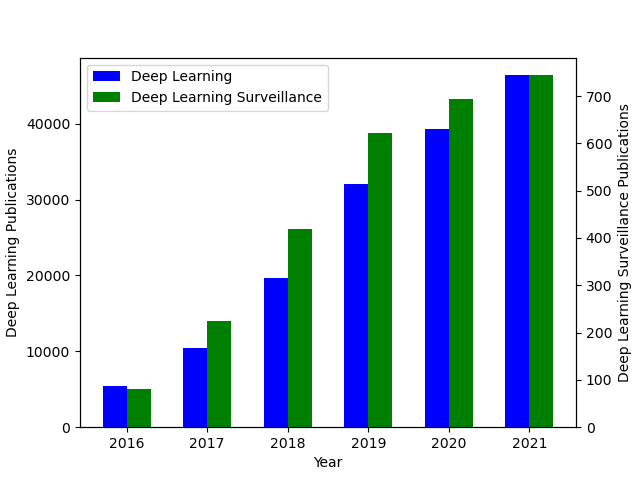
\includegraphics[width=\linewidth]{resources/introduction/publications_graph}
    \caption[Publications Increase Comparison]{The increase in publications mentioning the terms "deep learning" and "deep learning surveillance"~\cite{deep_learning_surveillance_stats}.}
    \label{fig:dl_publications}
\end{figure}
Yet despite major progress within the field of deep learning, there are still many tasks where humans outperform deep learning models, especially in anomaly detection where the nature of anomalies is typically difficult to define. Deep learning approaches also perform poorly when dealing with noise and concept drift.
\par
The cause for the discrepancy lies in the difference between how humans and machine learning algorithms represent data and learn. Most machine learning algorithms use a dense representation of the data and apply back-propagation in order to learn. Human learning happens in the neocortex, where evidence points to that the neocortex uses a sparse representation and performs Hebbian-like~\cite{hebbian_learning} learning. For the latter, there is a growing field of machine learning dedicated to replicating the inner mechanics of the neocortex, namely  \gls*{htm} theory. This theory outlines its advantages over standard machine learning, such as noise-tolerance and the ability to adapt to changing data.
\par
With the advantages of  \gls*{htm} and the rise of video anomaly detection in mind, a natural question one could pose is whether it is possible to apply  \gls*{htm} for anomaly detection in videos. Combined with a lack of related works, it is this very question that is the motivation behind this thesis.

\section{Problem Statement}
\label{sec:problem_statement}
Based on the background and motivation, the problem statement can be boiled down to a simple question: \textbf{Is \gls*{htm} viable for use in video anomaly detection?}\par
This thesis will introduce three different objectives that will help answer the question and also showcase the performance of HTM. It will also cover all required knowledge. The objectives are as follows:
\begin{enumerate}
    \item \objective{1}
    \item \objective{2}
    \item \objective{3}
\end{enumerate}

\section{Limitations}
HTM is a complex topic not part of the curriculum in most educations, if any at all. It is also based on neurological research, lending terms and concepts from the biological field, which significantly raises the barrier to entry for people with a machine learning background. The field also has a low level of accessibility due to a lack of proper documentation and a high reliance on the comparatively small \gls*{htm} community. This makes learning and understanding \gls*{htm} a process which takes up a sizable chunk out of the total time spent on this thesis. As such, this thesis will be relatively limited in scope, and will therefore focus mainly on anomaly detection in the context of surveillance.
\par
Additionally, \gls*{htm} for video anomaly detection~\cite{MotionAnomalyDetection} is a novel topic and is therefore naturally limited on several fronts. One of the main limitations is the lack of labeled anomaly data that suits the nature of HTM, because most datasets are made for use with deep learning approaches. Deep learning video datasets usually consist of many short segments whereas HTM suitable video datasets would consist of continuous videos, which was proven to be hard to come by during the work of this thesis. The main experiment of this thesis will therefore focus on only one dataset, due to the absence of suitable alternatives.
\par
There is also a lack of works related to applying \gls*{htm} on video-based problems, as  well as a lack of other methods that can be used for video anomaly detection that are based on the same premises as HTM. This means that there is a major lack of methods to use for the purpose of benchmarking and comparison.
\par
It should also be mentioned that the \gls*{htm} theory described in this thesis is not the first generation~\cite{htm_zeta1}, which was probabilistic in nature. The \gls*{htm} theory described in this thesis is actually the third generation~\cite{htm_gen3, thousandbrains}, which builds upon the second generation~\cite{htm_gen2_sp,htm_gen2_tm}. The second generation is often referred to as Cortical Learning Algorithms (CLA), which made the move from probabilistic modelling to Sparse Distributed Representation. The third generation builds upon the second generation by introducing concepts such as sensorimotor inference and The Thousand Brains Theory. The first generation had fundamentally different inner workings, but shared a lot of the terms with the current generation. This has made researching  \gls*{htm} challenging as there are many research papers published that refer to the first generation.
\par
Finally, it needs to be noted that Numenta, which is the company behind HTM, is a private for-profit company. This means that it is in their best interest to present \gls*{htm} as a highly functional and powerful machine learning algorithm. This can lead to unhealthy optimism, which has caused complications during the work of this thesis. One should therefore be critical when reading research papers from Numenta, and always keep in mind that they might not only be research papers but may also be marketing materials. It should also be mentioned that this thesis is relying on the community fork~\cite{htm_community_fork} of \gls*{htm} because Numenta has stopped development on the original codebase.

\section{Contributions}
This thesis explores the use of \gls*{htm} for anomaly detection in videos, and introduces a new type of \gls*{htm} architecture called Grid HTM, which requires a vigorous understanding of HTM. The main contributions are therefore achieved through the objectives introduced in \autoref{sec:problem_statement}. How this thesis achieves those objectives is described below:
\paragraph*{Objective 1} \emph{\objective{1}}
\par
This objective is achieved in \autoref{sec:background}, where \gls*{htm} is explained. This chapter also acts as an organization of  \gls*{htm} related research, supported with visualizations and a simpler language, making it easier for people with a machine learning background to understand. It is also important to mention that not only does this chapter include the main \gls*{htm} research published, but it also contains little tidbits of community research and ideas which are otherwise hard to come by.
\paragraph*{Objective 2} \emph{\objective{2}}
\par
This objective is achieved in \autoref{sec:grid_htm}, where Grid \gls*{htm} is introduced. Not only does it present a novel way to apply  \gls*{htm} on video-based problems, it also uncovers the reasoning behind the design decisions that were made as well as providing thorough analysis. This objective is further achieved through the Grid HTM paper, which is a product of this thesis, and can be found in \autoref{appendix:paper}.
\paragraph*{Objective 3} \emph{\objective{3}}
\par
This objective is achieved in \autoref{sec:experiments}, where three different experiments are performed. The first experiment showcases that \gls*{htm} and Grid \gls*{htm} can indeed perform anomaly detection on simple and clean videos. The second experiment showcases the performance of Grid \gls*{htm} on a complex surveillance video, which shows promising results. The third experiment showcases the ability of Grid \gls*{htm} to detect segments in a video, where noisy videos of sperm are used for increased challenge.
\par
With the three objectives achieved, it is possible to answer the thesis question: \textbf{Is \gls*{htm} viable for anomaly detection in videos?} The experiments show that with proper data and further refinements, Grid \gls*{htm} and other \gls*{htm} based architectures can indeed be used as anomaly detection systems for videos. However, as mentioned earlier, there is a lack of approaches to compare against which makes it hard to quantify the relative performance of Grid HTM.
\par
Additionally, during the course of this thesis, a contribution has been made to the  \gls*{htm} community in the form of uncovering and reporting a bug related to the technical implementation of  \gls*{htm}~\cite{github_contrib}. It is also important to reiterate that this thesis acts as a general guide to \gls*{htm} from a machine learning perspective, which is something that is sorely needed due to the low accessibility of the \gls*{htm} field.
\par
Finally, the work done in this thesis has produced a paper which can be found in \autoref{appendix:paper}. The work, including the Grid \gls*{htm} source code and the various experiments, is publically available on Github~\cite{master_thesis_github}.
\section{Research Methods}
Due to the novelty of this thesis, a single research method could not be used. Instead, a combination of multiple research methods was employed. For most of the thesis, an exploratory research method~\cite{exploratory_research} was used with the context of answering the thesis question, this was used due to the novelty of this thesis and the lack of related works. The result of this exploratory method is Grid HTM, which began from a simple starting point and was shaped through exploring improvements and solutions to problems that arose.
\par
For the surveillance experiment, a qualitative research method~\cite{quantitative_qualitative} was used to determine the effectiveness of Grid HTM. This is due to the lack of labeled data which made it hard to quantify, and that real life surveillance examples are complex by nature. The result is that the effectiveness was determined not through numbers, but through whether the results were qualitatively reasonable.
\par
As for the other experiments, a more quantitative research method~\cite{quantitative_qualitative} was used. This was made possible in the bouncing ball experiment due to the controlled nature of the experiment. In the sperm experiment, this was made possible due to the use of a benchmark, which allowed for direct comparisons.
\section{Thesis Outline}
This thesis consists of five chapters, where \autoref{sec:introduction} and \autoref{sec:background} are introductory and contain relevant background information for the understanding of the proceeding chapters. \autoref{sec:grid_htm} and \autoref{sec:experiments} present the work done during this thesis. \autoref{sec:conclusion} summarizes this thesis and presents areas in which there can be performed further work. More details for each of the chapters, except this one, is presented below.
\par
\subsection*{Chapter 2: Background}
\autoref{sec:background} covers the required knowledge for the proceeding chapters, as well as a short section about ethical considerations. It is split up into three parts. The first part covers deep learning and its history, and has an increased focus on the parts of deep learning that are especially relevant for this thesis, such as generative models.
\par
The second part covers anomaly detection. More specifically, it covers the definition, challenges, and recent work within anomaly detection. It also discusses smart surveillance, which is a subset of anomaly detection specifically meant for surveillance purposes.
\par
The third and final part covers \gls*{htm} theory. It starts off by introducing the biological ties to \gls*{htm} and the pipeline of an \gls*{htm} model. This is then proceeded by a detailed account of the inner mechanisms of an \gls*{htm} model and how learning is performed. It then finishes by introducing use-cases, related work on the use of \gls*{htm} for anomaly detection and how it performs, and highlights similarities between recent developments within \gls*{htm} theory and recent developments within deep learning.
\subsection*{Chapter 3: Grid HTM}
This chapter introduces Grid HTM, a novel \gls*{htm} architecture for the purpose of anomaly detection in videos, which is the main contribution of this thesis.
\par
Grid \gls*{htm} is presented gradually as problems occur and have to be solved. Some of these problems are invariance and unstable anomaly output. The technicalities are explained with the help of figures and various analyses. This architecture is then used in \autoref{sec:experiments} when performing experiments.
\par
Potential use cases are presented, such as reducing the need for expensive live monitoring as well as anomaly data labeling. The biological plausibility is also briefly discussed, and concludes that Grid \gls*{htm} may loosely be considered a cortical region.
\subsection*{Chapter 4: Experiments and Results}
This chapter presents three experiments that aim to explore the capabilities and challenges of \gls*{htm} and Grid \gls*{htm} in the context of anomaly detection in videos. The first experiment is a controlled experiment where a computer-generated ball is bouncing with anomalies inserted. The aim of this experiment is to test whether the capabilities of \gls*{htm} apply for videos, as well as the performance of Grid \gls*{htm} on the same task.
\par
The second experiment showcases the performance of Grid \gls*{htm} on a surveillance video with technical anomalies. Additionally, several key points of interests and the respective outputs of Grid \gls*{htm} are shown in order to get a better understanding of its capabilities.
\par
The third experiment further explores the ability of Grid \gls*{htm} to detect segments in videos, which was discovered in the previous experiment. The videos that are used in this experiment are videos of sperm that contain several segments.
\subsection*{Chapter 5: Conclusion and Further Work}
In this chapter the thesis is summarized, and the thesis question presented in \autoref{sec:introduction} is answered along with potential further work, as well as the main contributions of this thesis.
\par
The contributions are presented as the description of how the various objectives were achieved, as well as answering the thesis question. This is a shorter version of the contributions mentioned in the introduction, and is presented conclusively.
\par
This chapter also presents potential future work, which is further divided into sections focusing on different aspects such as datasets, Grid HTM, HTM and deep learning, and general research progress.
\chapter{Background}
The following is relevant background information on HTM theory, Deep Learning, and Video Anomaly Detection.
\section{Deep Learning}
As mentioned in the introduction, deep learning has seen increased popularity for the past few years. Surprisingly enough, the field of deep learning can be traced back to 1958 when the Perceptron\cite{perceptron,perceptron2} was first introduced.
\subsection{Perceptron}
The perceptron\cite{perceptron, perceptron2} was a machine learning algorithm that was based off a simplification of the theory, at the time, on how a neuron worked. The perceptron consists of three parts; the inputs $\mathbf{x}$, the weights $\mathbf{w}$, and the unit step activation function.
\begin{figure}[H]
    \centering
    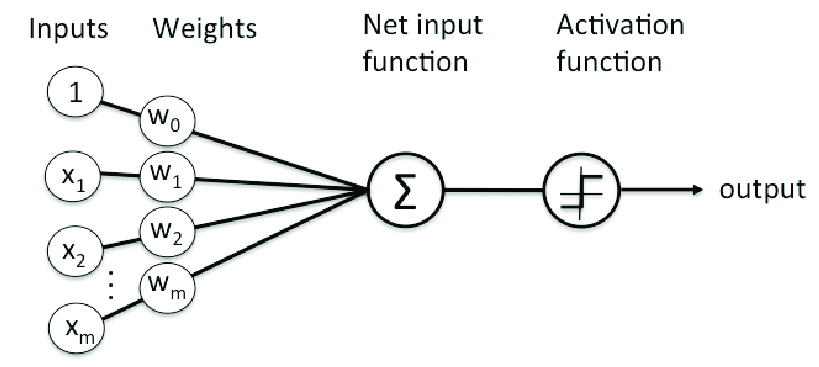
\includegraphics[width=0.6\linewidth]{resources/related_works/perceptron.png}
    \caption{Perceptron}
\end{figure}
It also requires a label $y$ corresponding to the input $\mathbf{x}$. The perceptron predicts the label of the input $\mathbf{x}$ to be $\hat{y}=sign(\mathbf{x}\cdot\mathbf{w})$. If $\hat{y}\neq y$ then it updates the weights $\mathbf{w}=\mathbf{w}+y\mathbf{x}$, otherwise it leaves $\mathbf{w}$ unchanged. This is performed until the perceptron reaches convergence, which would happen when all the inputs can be correctly classified. In other words, the perceptron requires that the inputs are linearly separable.
\par
As shown by \textcite{perceptron3}, the perceptron was able to solve linearly separable problems such as the OR function, but was unable to solve the XOR function. For the latter, it was theorized by others that stacking perceptrons in multiple layers, known as a \gls*{g_mlp}, would be able to solve more complex problems such as the aforementioned XOR function\cite{perceptron_misconceptions}. Unfortunately, the work by \textcite{perceptron3} lead to the misconception that \glspl*{g_mlp} would have the same limitations as a single perceptron, and that further progress was impossible which lead to the perceptron and other neuron-based approaches being largely abandoned\cite{perceptron_misconceptions}. This misconception, combined with a lack of computing power and no good approaches to train a \gls*{g_mlp}, lead to a decline in the research of neuron-inspired approaches.
\begin{figure}[H]
    \centering
    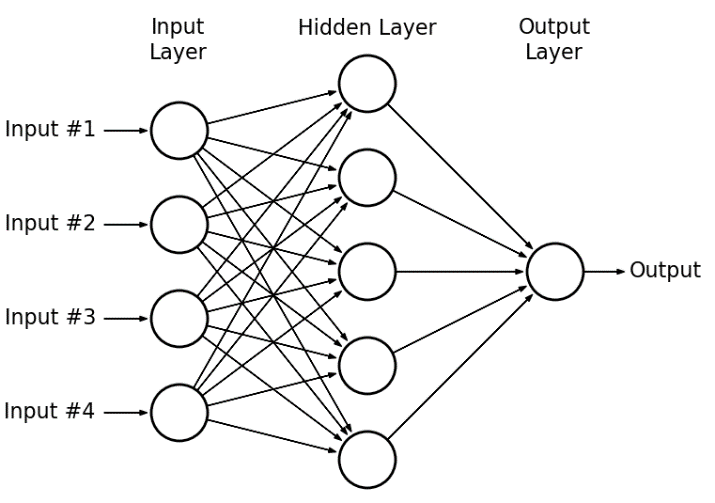
\includegraphics[width=\linewidth]{resources/related_works/mlp.png}
    \caption{Example of a MLP. Source: \cite{mlp_image}}
\end{figure}
\par
It was not until the late 1980s\cite{perceptron_misconceptions} that the \gls*{g_mlp} approach experienced a revival, led by the increase in computational power and the introduction of backpropagation by \textcite{backprop}, which allowed multilayer networks to be easily trained, and gave birth to modern neural networks.
\subsection{Backpropagation}
Backpropagation\cite{backprop}, which is shorthand for "backward propagation of errors",  is a method for efficiently calculating the gradient of the error function, so that it is possible to adjust each individual weight with the purpose of lowering the error. The error function is a function that quantifies the difference between a prediction and the corresponding label, and is differentiable. An example of such an error function, is the \gls*{g_mse}:
\begin{align*}
    MSE=\frac{1}{n}\sum_{i=1}^n (y_i-\hat{y}_i)^2
\end{align*}
The result is that no longer did researchers have to manually engineer features, but could instead apply backpropagation to have the neural network automatically learn internal representations that expressed nontrivial features. An example is that in an image, a collection of pixels could be represented as a line.
\subsection{Neural Networks}
Modern \gls*{g_mlp} networks, often referred to as just "neural networks", are similar to what was theorized earlier. The main difference is that each neuron in a \gls*{g_mlp} can have an arbitrary activation function, such as the sigmoid function and the \gls*{g_relu}\cite{relu} function, which adds nonlinearity into the neural network and allows it to solve complex problems. They also contain more hidden layers, in other words they are "deeper", hence the name "deep learning".
\begin{figure}[H]
    \centering
    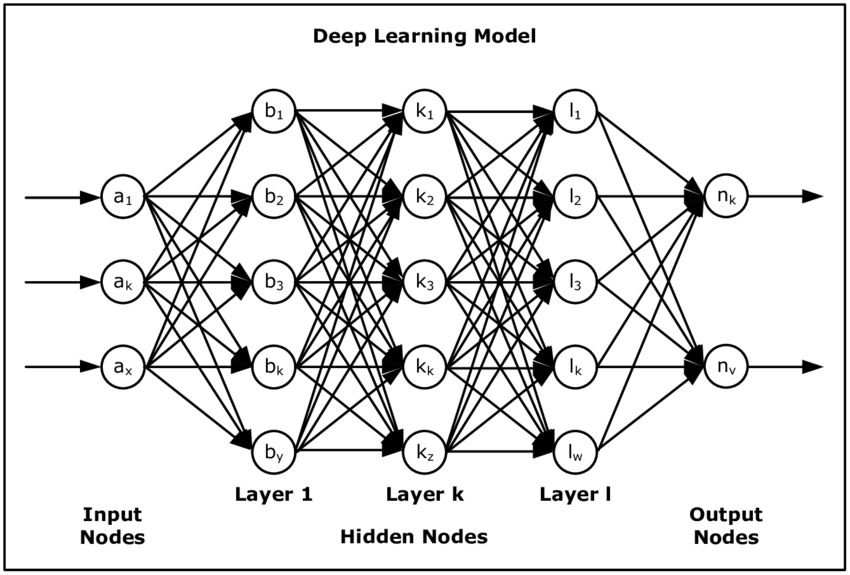
\includegraphics[width=\linewidth]{resources/related_works/nn.png}
    \caption{Example of a neural network. Source: \cite{nn_image}}
\end{figure}
The gradients are calculated using backpropagation which are then used by optimization methods to update the weights with the goal of reducing the error. Examples of optimizers are \gls*{g_sgd}\cite{sgd} and AdamW\cite{adamw}.
\begin{figure}[H]
    \centering
    \includegraphics[width=0.6\linewidth]{example-image-a}
    \caption{Gradient Descent}
\end{figure}
\par
Yet with all the advancements within the field of neural networks, it still did not have the popularity that can be observed today. There are several reasons for this, one of them arguably being the introduction of Support Vector Machines (SVM)\cite{svm}, which put neural networks in the background.
\par
The other reason is that neural networks did not have a lot of applications at the time, this being due to a lack of invariances which caused poor performance in machine vision, and no proper way to represent features across time which caused poor performance in time-series analysis. There was also a lack of regularization methods, which caused the models to overfit, and generalize poorly. Additionally, large networks suffered from vanishing or exploding gradients.
\par
In order to improve upon regularization, techniques such as Dropout\cite{dropout}, \gls*{g_bn}\cite{batchnorm}, and data augmentation\cite{data_augmentation} were introduced. New neural network architectures were invented, such as the Autoencoder\cite{autoencoder}, that forces the model to construct an internal representation under constraints which has a regularizing effect.
\par
As for representing features across time, architectures such as \glspl*{g_rnn}\cite{lstm,gru} and later attention\cite{attention}-based models such as Transformer\cite{transformer} models were created.\par
The vanishing/exploding gradient problem was alleviated by implementing residual connections\cite{resnet} between layers, among other techniques.
\subsection{Convolutional Neural Networks}
In an attempt to solve the problems regarding invariance and to improve the performance in machine vision tasks, \glspl*{g_cnn} were introduced by \textcite{cnn} in 1998. A \gls*{g_cnn} offers several properties that are useful, such as translational invariance \cite{cnn}. These properties stem from the three architectural ideas in a CNN:
\begin{itemize}
    \item Local receptive fields
    \item Shared weights
    \item Spatial sub-sampling
\end{itemize}
Through the use of data augmentation, it is also possible to not only improve the effectiveness of the aforementioned invariances, but to also introduce a degree of rotational and scale invariance.
\begin{figure}[H]
    \centering
    \includegraphics[width=0.5\linewidth]{example-image-a}
    \caption{CNN}
\end{figure}
\par
However, the progress, in the context of machine vision, stagnated due to a lack of computing power when training on large datasets. This stagnation lasted until 2012 when AlexNet was introduced by \textcite{alexnet}, which marked a major turning point in the history of deep learning, as their results proved that deep learning was they way forward for solving advanced problems.
\par
In addition to creating a unique \gls*{g_cnn} architecture, they also made it run on a GPU and made the code publicly available. This was not the first case of running deep learning on a GPU\cite{deeplearning_gpu}, but it can be argued that it was this paper that popularized it.  Using GPUs meant that a vast amount of computational power, for the purpose of training deep learning models, became unlocked. This also paved the way for frameworks such as PyTorch\cite{pytorch} and Tensorflow\cite{tensorflow}, which have democratized deep learning and made it into what it is today.
\subsection{Generative Models}
Some of the latest progress within deep learning can be contributed to generative models, such as \glspl*{g_gan}\cite{gan} and \glspl*{g_vae}\cite{vae}. Generative models work by taking some input, and then generating realistic output. The input could be anything from random noise to a real sample. The idea is that the models learn a distribution which describes the data domain represented by the training data, and can then generate synthetic data from that distribution by simply sampling it.
\subsection{Disadvantages}
A disadvantage for deep-learning models in general is that they are susceptible to noise in the dataset \cite{noise1,noise2}. They are also in most cases not self-supervised and therefore require constant tuning in order to stay effective on changing data. Not to mention that they require a lot of data before they can be considered effective. They also suffer from issues with out-of-distribution performance. Susceptible to noise in the data. Also issues with explainability.
\subsubsection{Explainability}
As stated by \textcite{XAI}, as "black-box" approaches such as deep learning surged in popularity, many realized that they offered poor explainability. While it is known \textit{how} the models make their decisions, their huge parametric spaces make it unfeasible to know \textit{why} they decide as they do. Combined with the vast potential that deep learning offers in critical sectors such as medicine, has lead to an increase in focus on developing approaches that offer explainability.
\begin{figure}[H]
    \centering
    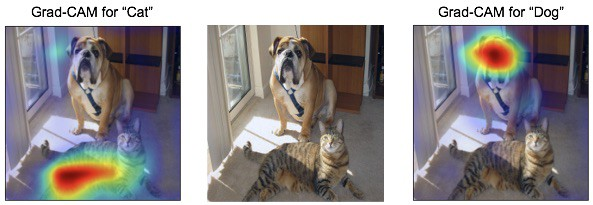
\includegraphics[width=\linewidth]{resources/related_works/gradcam.jpg}
    \caption{Grad-CAM visualization for cat and dog.}
\end{figure}
Approaches such as Grad-CAM \cite{GradCAM} and Guided Backpropagation \cite{guided_backprop} offer improvements in that regard, but these approaches are not made with generative models in mind. In fact, there are very few explainable AI approaches for generative models \cite{XAI}.
\section{Anomaly detection}
As reviewed by \textcite{anomaly_detection}, anomaly detection is often defined as detecting data points that deviate from the general distribution of the data, this also often includes quantifying the level of deviation. Unlike other problems within machine learning and statistics, anomaly detection deals with unpredictable and rare events, therefore adding complexities to problems. Some complexities are as follows:
\begin{itemize}
    \item \textbf{Unknowns} Anomalies are associated with many unknowns which do not become known until the anomaly happens. \cite{unknown_detection1,unknown_detection2} are works that address this.
    \item \textbf{Rarity and class imbalance} Anomalies are by definition rare instances, which means that it becomes difficult to create a balanced dataset. \cite{class_imbalance1} reviews the current solutions to this problem.
    \item \textbf{Heterogeneity} Anomalies can take form in many ways, and as such one class of anomalies can be vastly different from another. Approaches such as \cite{heterogeneous1} have been proposed to alleviate the problem.
\end{itemize}
This makes it hard to apply traditional deep learning methods for anomaly detection, because they are designed with pairs of $\{input, target\}$ in mind.
\subsection{Deep Learning and Anomaly Detection}
The current state-of-the-art algorithms for anomaly detection are numerous, but the main approach is achieved by using deep learning \cite{anomaly_detection}. As previously mentioned, traditional deep learning approaches are hard to apply for anomaly detection. Instead, a popular approach is to use generative deep learning models such as GANs \cite{anomaly_detection, ganomaly,anomalyvideo} to generate synthetic data and compare it to real data in order to detect anomalies. This approach is based on the assumption that the model will only be able to generate data similar to what it has been trained on, and therefore fail when an anomalous event occurs.
\par The advantage is that GANs are generally good at generating realistic data, especially when it comes to images. The disadvantage is that GANs are very hard to train and may give suboptimal results given that it tries to generate good synthetic data rather than directly detect anomalies. The training data also needs to contain all possible non-anomalous classes of events, which may not be a realistic expectation.
\par
\begin{figure}[H]
    \centering
    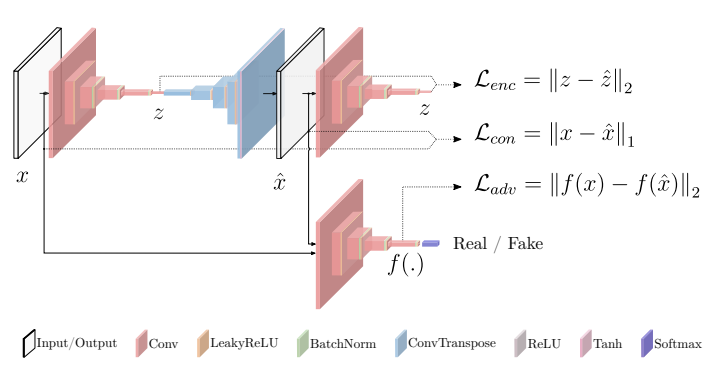
\includegraphics[width=\linewidth]{resources/models/ganomaly.png}
    \caption{GANomaly \cite{ganomaly}, a variation of GAN for Anomaly detection}
    \label{fig:ganomaly}
\end{figure}
Another common approach is autoencoders, which aim to minimize the reconstruction error from a learned feature representation space \cite{autoencoder1,anomaly_detection,anomalyvideo}. The assumption is that anomalies are more difficult to reconstruct than normal data, hence the reconstruction error will be high and can therefore be used as a metric to detect anomalies.
\par
Additionally, they are very hard to design and train for the purpose of detecting anomalies in complex data such as surveillance. As previously stated, since generative models make up most of the state-of-the-art approaches in anomaly detection, this means that there is a lack of explainability in the field of anomaly detection in videos.
\par
There are also variations of the aforementioned approaches, such as Adversarial Autoencoders, but the core idea is the same; to get an anomaly measure using some sort of generated or reconstructed data.
\subsection{Smart Surveillance}
Smart surveillance, which is the use of automatic video analysis in surveillance, has seen rapid development since its inception. \cite{anomalyvideo} presents and summarizes recent progress for anomaly detection in video for surveillance purposes, where the most promising methods are achieved by using convolutional auto-encoders (AE) and Generative Adversarial Networks (GAN). The results show that the deep learning approaches have a high degree of accuracy, and are consistently improving. \par
The paper also discusses problems with using deep learning approaches for anomaly detection. One of the examples that it uses is about a bicycle on campus being wrongly classified as an anomaly, which is related to the aforementioned issue with the non-realistic requirement that the training data must contain all possible classes of non-anomalous events.

\section{Hierarchical Temporal Memory}
Today's machine learning algorithms aim to solve complex problems by simulating a substantial amount of mathematically defined neurons. These neurons are vastly simplified compared to the neurons in the brain and therefore do not have the complexity required to solve complex problems with an accuracy and level of generalizability comparable to the brain. \textcite{BAMI} introduces HTM theory which aims to outline a machine learning algorithm which works on the same principles as the brain and therefore solves some of the aforementioned issues.\par
The brain consists of layers that have been added throughout evolution. The inner layers are responsible for primal intelligence such as hunger, sex and instincts. HTM theory specifically aims to simulate the neocortex which is the outer layer of the brain tasked with advanced logic. It is important to note that HTM only attempts to estimate the activity in the brain, unlike Spiking Neural Networks and others which aim to accurately simulate the activity of the brain \cite{spiking_neural_networks}.
\subsection{Structure}
HTM aims to replicate the structure of the neocortex which is made up of cortical regions. Cortical regions consist of cortical columns, where each column is divided into layers height-wise. These cortical columns are made up of mini-columns, which in turn are made up of neurons.
\begin{figure}[H]
    \centering
    \begin{subfigure}{0.6\textwidth}
        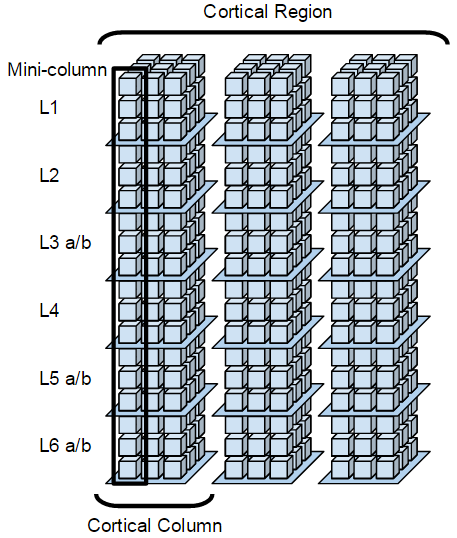
\includegraphics[width=\textwidth]{resources/related_works/cortical_region.png}
        \caption{Cortical Region.}
    \end{subfigure}
    \hfill
    \begin{subfigure}{0.35\textwidth}
        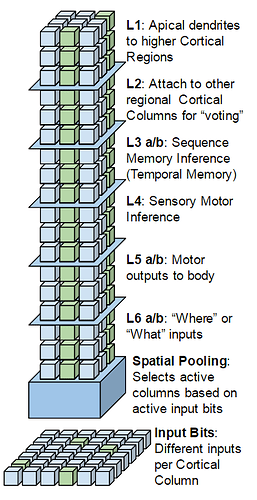
\includegraphics[width=\textwidth]{resources/related_works/cortical_column.png}
        \caption{Cortical Column.}
    \end{subfigure}

    \caption{Visualization of the cortical region structure in the neocortex according to HTM theory. Note that current HTM implementations only model L2/L3, but can be extended to model L4 as well \cite{htm_l2_l3}. Source: \cite{cortical_region}}
    \label{fig:cortical_region}
\end{figure}
Neurons in HTM theory are different from neurons in traditional machine learning. The term neuron in traditional machine learning is very misleading and since it is mathematically derived, has actually very little in common with a biological neuron. A biological neuron does not perform back propagation but learns by strengthening and weakening inter-neural connections (synapses), which is something that the HTM neuron attempts to model through Hebbian like learning.
\begin{figure}[H]
    \centering
    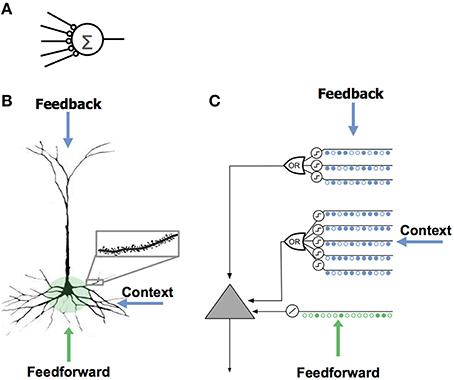
\includegraphics[width=\linewidth]{resources/related_works/neuron_comparison.jpg}
    \caption{Comparison of neurons \protect\cite{htm_neurons}: Traditional Machine Learning (A), Biological Neuron (B), HTM Neuron (C). Source: \cite{BAMI}}
    \label{fig:neuron_comparison}
\end{figure}
The HTM neuron has three inputs \cite{htm_neurons}:
\begin{itemize}
    \item Feedforward, which is the input data
    \item Context, which is data from neighboring neurons and acts as a prediction mechanism for the next feedforward input
    \item Feedback, which is feedback from other neurons in the hierarchy and acts as a prediction mechanism for a sequence of feedforward inputs
\end{itemize}
How this type of neuron operates will be covered in greater detail later in this section.
\subsection{Common Algorithm}
HTM theory states that there is a common algorithm for the intelligence. That the signals from hearing, vision, and touch are at the core processed by the same common algorithm. By extension, this means that HTM networks should be able to solve all kinds of logical tasks.
\subsection{Sparse Distributed Representation}
HTM theory introduces Sparse Distributed Representation (SDR) as a way of representing data in HTM and can be thought of as a bit-array. Each bit theoretically corresponds to a neuron in the neocortex and also represents some semantic information about the current data. This opens up for all kinds of mathematical operations, for instance it is possible to compare the semantic similarities between two SDRs by simply performing a binary AND operation.
\begin{figure}[H]
    \centering
    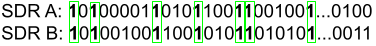
\includegraphics{resources/related_works/sdr-semantics.png}
    \caption{Semantic similarities between the two SDRs A and B}
    \label{fig:sdr_semantics}
\end{figure}
Observations of the brain has found that at any given point in time, a small percentage of neurons are activated and an SDR aims to keep this property by having a small percentage of bits be 1 at any given point. A common value is 2\% in order to mimic the sparsity of active neurons in the neocortex. Having this property means that the chance of two bit-patterns with different semantic meanings coinciding, for instance due to bit-flips caused by noise in the data, is astronomically low and is what makes HTM robust to noise.
\begin{figure}[H]
    \centering
    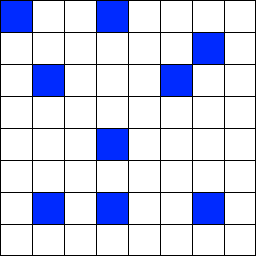
\includegraphics[width=0.25\textwidth]{resources/related_works/SDR.png}
    \caption{Example representation of an SDR with a length of 64 and a sparsity of 14.1\%, visualized as a 2D grid.}
\end{figure}
\subsection{Encoders}
To convert real-world data into an SDR, there is a need for an encoder in the pipeline. These encoders can be designed to take potentially any data and convert it into an SDR with an arbitrary sparsity. Given the fact that they may have an arbitrary sparsity, the output SDRs created by the encoder are sometimes referred to as just binary arrays.\par
Writing an encoder is no easy task as it is important to keep semantic similarities between values. This also means that the encoder is perhaps the most important part of an HTM pipeline to get right as it is the part that can limit the system the most.\par

A biological example would be an eye that takes in visual information and converts it into an SDR so that it can be processed by the neocortex. This is the most important part for this thesis as creating a high dimensional encoder for video is still being researched.\par
There are principles that should be followed in order to create a good encoder:
\begin{itemize}
    \item Semantically similar data should result in SDRs with overlapping active bits
    \item The same input should always produce the same SDR
    \item The output must have the same dimensionality (total number of bits) for all inputs
    \item The output should have similar sparsity (similar amount of one-bits) for all inputs and have enough one-bits to handle noise and subsampling
\end{itemize}
As of now, there exists encoders for numbers, categories, geospatial locations, and dates.
\begin{figure}[H]
    \centering
    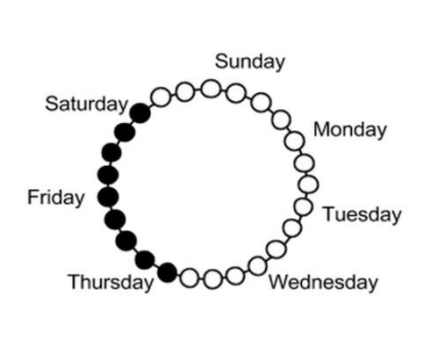
\includegraphics[width=0.55\linewidth]{resources/related_works/cyclical_encoder.png}
    \caption{Visualization of a cyclical date encoder, which is currently encoding Friday. Note that also Thursday and Saturday are included in the encoding of Friday in order to emphasize that Thursday and Saturday are both equally distanced from Friday. Source: \cite{BAMI}}
    \label{fig:cyclical_encoder}
\end{figure}
Some applications may require anomaly detection on multiple values at once, the correct approach then is to encode the values one by one and then concatenate them into a single SDR before passing it to the HTM.
\par
Several approaches for encoding visual data have been proposed, such as \cite{eyeencoder} which uses a neuroscientifical approach by replicating how the eye works, and \cite{ObjectDetectionSIFT} which uses scale-invariant feature transform (SIFT) to find points of interest in images and encode that information as an SDR. There are also deep learning approaches such as \cite{CNN_HTM} which uses a Convolutional Neural Network (CNN) as part of the encoder, specifically they use the top $n$-features in a feature map as ones and set the rest to zeros in order to construct their SDRs.
\par
The reason for why a direct binary encoding might not perform well is due to the fact that it is neither position nor scale invariant and as such breaks the first principle of creating a good encoder. For instance, if it is desired that two pictures of the same object, but in different scales have more or less the same semantic meaning, then a direct binary encoding is not going to work. Direct binary encodings also lead to loss of information, and is hard to perform for complex objects.
\begin{figure}[H]
    \centering
    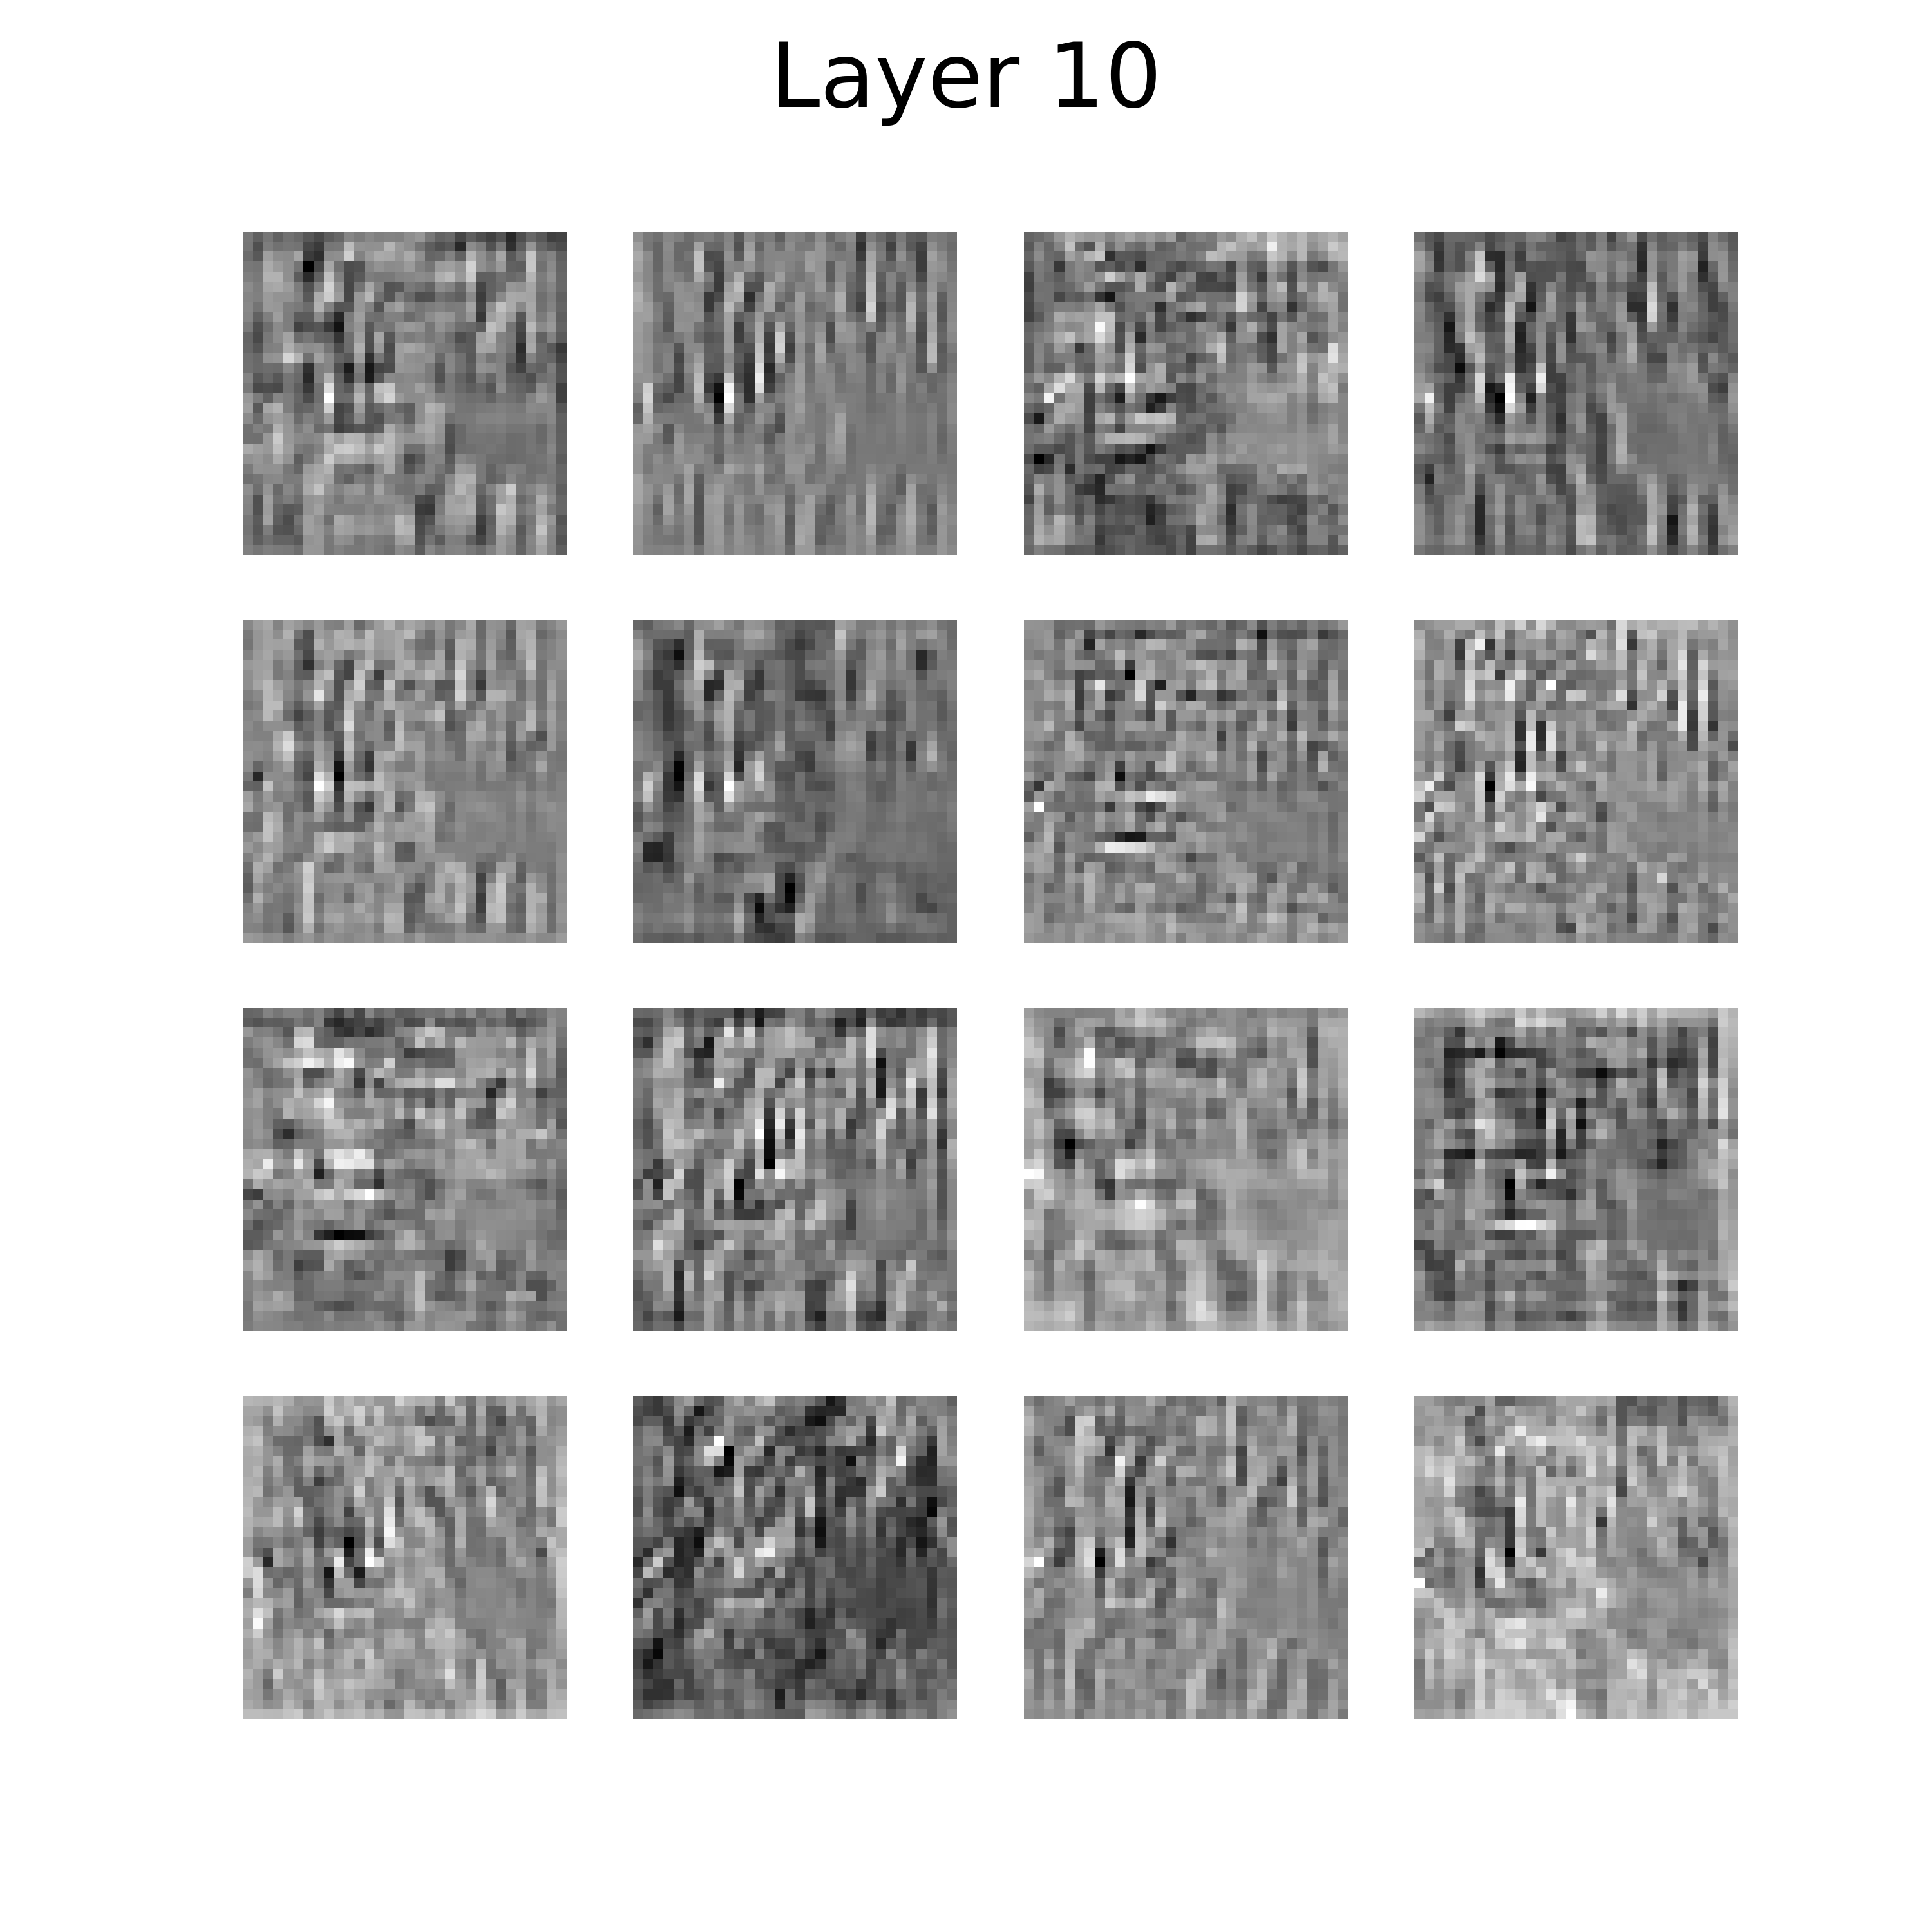
\includegraphics[width=\linewidth]{resources/related_works/resnet18_layer_10.png}
    \caption{Select few feature map activations in the 10th layer of ResNet18\cite{resnet} trained on ImageNet\cite{imagenet}.}
    \label{fig:cnn_features}
\end{figure}
\par
An encoder which transforms convolutional feature maps into SDRs could help solve this, but the issue is converting the dense representation of the feature maps into SDRs. Directly encoding them into SDRs by treating each value in the feature map as a float and converting it into its own SDR quickly becomes intangible due to the processing and memory requirements. \autoref{fig:cnn_features} shows only a small subset of all the feature maps in a single layer, which highlights how intangible this approach is.
\par
Additionally, minor variations in the feature map would cause major variations in the resulting SDR. Alternatively, one could follow \textcite{CNN_HTM} and binary threshold the top-$n$ features, but this leads to its own problems such as loss of information and that the information contained in the top-$n$ features is often undefined in models trained for complex tasks. It is also undefined what the top-$n$ features represent when there are no strong activations.
\subsection{Learning}
Similar to biological beings, HTM is designed to work on streaming data. It does not operate with batches like traditional machine learning, but rather with streaming data that may be changing over time. \par
The learning mechanism consists of two parts; the Spatial Pooler (SP) and the Temporal Memory (TM) algorithm. The latter is also commonly referred to as Sequence Memory. Together they make up the HTM neuron.\par
The spatial pooler takes SDRs produced by the encoder, and uses Hebbian like learning to extract semantically important information into output SDRs. These output SDRs usually have a fixed sparsity of about 2\% due to the fact the spatial pooler aims to produce SDRs that have similar sparsity to what has been observed in the neocortex, but this can be configured at will and is dependent on the problem at hand.\par
The temporal memory algorithm, on the other hand, simulates the learning algorithm in the neocortex. It takes the SDRs formed by the spatial pooler and does two things:
\begin{itemize}
    \item Learns sequences of SDRs formed by the spatial pooler
    \item Forms a prediction, in the form of a predictive SDR,  given the context of previous SDRs
\end{itemize}
\begin{figure}[H]
    \centering
    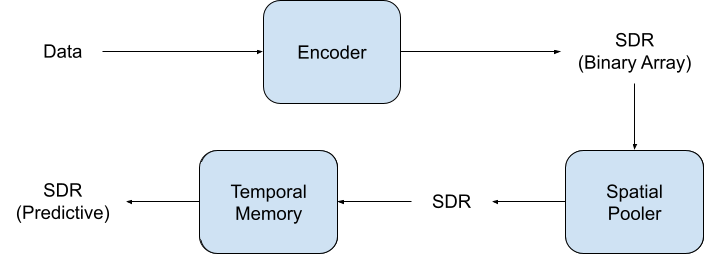
\includegraphics[width=\linewidth]{resources/related_works/htm_pipeline.png}
    \caption{The HTM Pipeline. A common next-step could be to use a classifier to convert the predictive SDR into a classification. }
    \label{fig:htm_pipeline}
\end{figure}

This gives HTM systems the property of on-line learning, meaning they learn as they go. There is no batch training because each input into the HTM system will update the system. The system effectively builds a predictive model of the data and learns by trying to minimize the error between the true values and the predicted values. This means that the system will continuously adapt to a changing environment.
\begin{figure}[H]
    \centering
    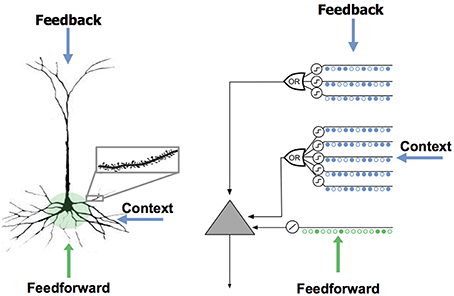
\includegraphics[width=\linewidth]{resources/related_works/htm_neuron.png}
    \caption{Real neuron and HTM neuron. }
    \label{fig:sp_tm_responsibility}
\end{figure}
\autoref{fig:sp_tm_responsibility} shows that a spatial pooler followed by a temporal memory forms the HTM neuron, where the color green indicates the responsibility of the Spatial Pooler and blue indicates the responsibility of the Temporal Memory.
\subsubsection{Spatial Pooler}
The spatial pooler consists of columns (mini-columns), where each column has a receptive field covering the input. In technical implementations of spatial poolers, the columns exist in name only and could be thought of as nodes instead. A column can cover parts of the input or the entire input, the range being referred to as the \textbf{potential radius}. During initialization, each column creates random connections to a percentage of the bits in the input space within its receptive field, this gives each column a unique \textbf{potential pool} when there are overlaps of receptive fields caused by a large potential radius.\par
\begin{figure}[H]
    \centering
    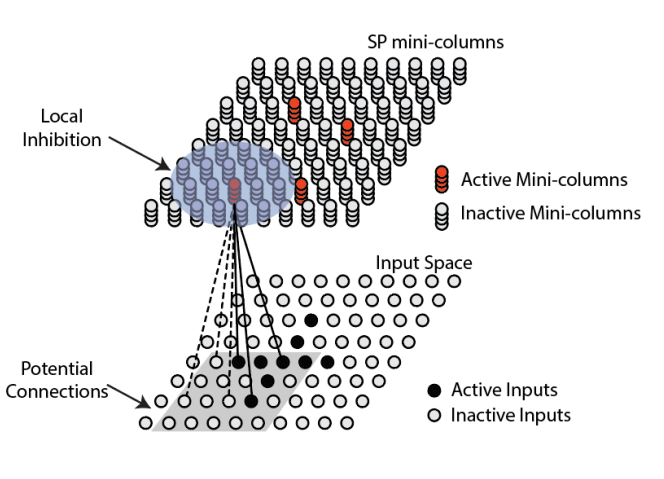
\includegraphics[width=\linewidth]{resources/related_works/sp_vis_alt.png}
    \caption{Visualization of the \gls*{sp} and the potential pool of one of its columns. Source: \cite{htm_sp_presentation}}
\end{figure}
Each connection is described using a \textbf{permanence}-value which can be considered the "strength" of the connection, and it ranges between 0 and 1. During learning, the permanence value of the connections is increased or decreased depending on whether the corresponding bit in the input is active or inactive. When the permanence-value crosses above a \textbf{stimulus threshold}, the connection will be considered "active".

The amount of active connections for a given column is referred to as \textbf{overlap score}. If a column has a high enough overlap score which crosses the \textbf{overlap score threshold}, then the column will itself become active. The reason behind locking activation behind a minimum overlap score is to reduce the influence of noise in the input. Finally, out of all the active columns, only the top $n$ columns with the most overlap score will be selected to be included in the \gls*{sp} output. The value $n$ is chosen so that the \gls*{sp} output has a specific \textbf{sparsity}. Only the selected columns are allowed to learn (increase/decrease permanence). \autoref{fig:sp_vis} visualizes the mechanism that determines the output in the SP.
\par
\begin{figure}[H]
    \centering
    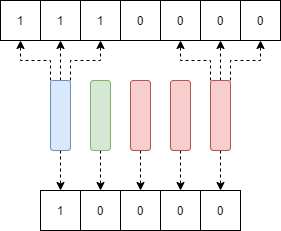
\includegraphics[width=0.6\textwidth]{resources/related_works/sp_vis.png}
    \caption{ This figure illustrates how a spatial pooler works. All connections are above the stimulus threshold. The receptive field is 3 bits wide for each column. Overlap score threshold is $1$, and $n=1$. Red means inactive, green means active, and blue means active and selected.}
    \label{fig:sp_vis}
\end{figure}
Because only the active columns are allowed to learn, only a select few columns who got lucky during the random initialization will dominate the spatial pooler output and have a very high \textbf{active duty cycle}. Active duty cycle measures how often a column is active and ranges from 0 (never) to 1 (always). \par
To counter dominating columns, the spatial pooler uses \textbf{boosting}.
The concept behind boosting it to "boost" the overlap score of underperforming columns and lower the overlap score of over performing columns. The result is that more columns learn and contribute to the output, which means that the spatial pooler can then process the input data with a finer granularity. One has to be careful with boosting, since it can cause instability in the spatial pooler output.
\par
It is also possible to have \textbf{topology} in the output by selecting the columns to be included in the output by their local neighborhood, instead of comparing their overlap score globally.
\par
All the aforementioned concepts are configurable in technical implementations.

\subsubsection{Temporal Memory}
\label{sec:temporal_memory}
The temporal memory consists of the columns that a spatial pooler outputs, but treats them as actual columns instead of "nodes". These columns consist of cells and can contain an arbitrary \textbf{number of cells} which defines the capacity of contexts that the temporal memory can express. Each cell in a column can connect to other cells in other columns using segments (more specifically, distal dendrite segments), where each segment consists of synapses connecting to other cells.
\par
Essentially, it takes the "node" based representation of the \gls*{sp} output, and turns it into a new representation which includes state, or context, from previous time steps. It achieves this by only activating a subset of cells per column, typically only one per column. This allows the temporal memory to represent a pattern in multiple contexts. If every column has 32 cells and the \gls*{sp} output has 100 active columns and only one cell per column is active, then the \gls*{tm} has $32^{100}$ ways of representing the same input. The same input will make the same columns active, but in different contexts different cells in those columns will be active.
\begin{figure}[H]
    \centering
    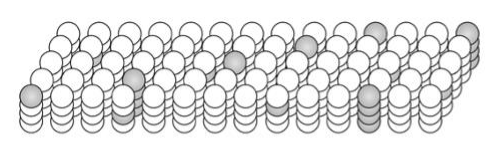
\includegraphics[width=\linewidth]{resources/related_works/tm_vis_alt2.png}
    \caption{Visualization of the TM, with number of cells equal 4. Some columns are bursting. Source: \cite{BAMI}}
\end{figure}
\par
The temporal memory algorithm consists of two phases. The first phase is to evaluate the \gls*{sp} output against predictions and choose a set of active cells. It does so by looking at the active columns and the cells they contain. If an active column contains predictive cells, then those cells are marked as active. If an active column has no predictive cells, usually caused by observing a new pattern for the first time, then the column "bursts" by activating all the cells that the column contains (see \autoref{fig:tm_vis1}). Otherwise, a cell is inactive.
\par
\begin{figure}[H]
    \centering
    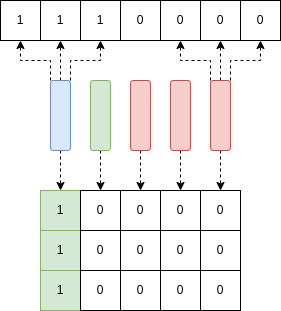
\includegraphics[width=0.6\textwidth]{resources/related_works/tm_vis1.png}
    \caption{Expanded \gls*{sp} example with \gls*{tm} component where the number of cells is set to 3. The leftmost column is bursting (all 3 cells activated in green) due to the active \gls*{sp} output and due to containing no predictive cells.}
    \label{fig:tm_vis1}
\end{figure}
At this point, the active cells represent the current input in the context of previous input. For each active column we look at the segments connected to the active cell(s). If the column is bursting we look at the segments that contain any active synapses, if there is no such segment we grow one on the cell with the fewest segments. On each of the segments that we are looking at, we \textbf{increase the permanence} on every active synapse, \textbf{decrease the permanence} on every inactive synapse, and grow new synapses to cells that were previously active. The algorithm also punishes segments that caused cells to enter predictive state, but which did not end up being active.
\par
Since the \gls*{tm} can only grow synapses to cells that were previously active, the \gls*{tm} struggles to express sequences of patterns over multiple timesteps, as has been discussed on HTM forums \cite{tm_sequence_problem}. The solution has been to also encode some temporal information, such as the time of day \cite{AHMAD2017134,tm_sequence_problem}, so that it can use timestamps as anchor points for its contexts.
\par
The second phase is to form a prediction by putting cells into a predictive state. For every segment on every cell, the number of synapses connected to active cells are counted. If the number exceeds an \textbf{activation threshold}, then the segment is marked as active and all the cells connected to the segment enter the predictive state. To summarize, a cell has three possible states:
\begin{itemize}
    \item Active, if the column is bursting or the cell was in a predictive state in the previous time step.
    \item Predictive, if a connected segment is active, which is in turn determined by the amount of active synapses.
    \item Inactive, if none of the other states apply.
\end{itemize}
\begin{figure}[H]
    \centering
    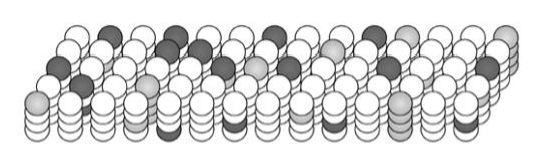
\includegraphics[width=\linewidth]{resources/related_works/tm_vis_alt.png}
    \caption{Visualization of the \gls*{tm} and the three states. Active in black, predictive in gray, and inactive in white. Source: \cite{BAMI}}
\end{figure}
One can configure how much the system can learn by setting the number of cells and the values by which permanence should be increased or decreased. If it is desired that the \gls*{tm} does not "forget" at all, then the permanence value by which synapses are decremented can be set to 0. If it is desired that the \gls*{tm} can only express patterns in the current context and the context of the previous time step, then the number of cells can be set to 2.
\par
Finally, the \gls*{tm} compares the predictions $P_{t-1}$ it made in the previous time step with the actual pattern $A_t$ in the current time step and calculates an anomaly score:
\begin{align*}
    anomalyScore=\frac{|A_t-(P_{t-1}\cap A_t)|}{|A_t|}
\end{align*}
Which is a normalized value from 0 to 1. If the anomaly score is 1, then it means that none of the predicted columns matched the current active columns of the spatial pooler. If it is 0, then it means that all predicted columns matched the current active columns of the SP.\par
It is also possible to estimate the number of predictions being made by the \gls*{tm} at any time \cite{htm_predictions_count}. This is done by counting the number of predictive cells, and dividing them by the number of active bits required to express a pattern. As an example, if sparsity is set so that patterns have 60 active bits and the number of predictive cells is 120, then the estimated number of predictions is given as
\begin{align*}
    numPredictions=\frac{predictiveCells}{activeBits}=\frac{120}{60}=2
\end{align*}
This is only an estimation, in reality the two patterns may have overlapping bits in their representations, and the number of active bits for each representation may have minor deviations.
\subsection{Use cases}
The general use case for HTM is to perform anomaly detection. More specifically, Numenta has made example applications showcasing how HTM can be used in practice \cite{numenta_example_apps}:
\begin{itemize}
    \item \textbf{Rogue Behavior Detection} which models normal behavior and detects anomalies, such as unusual use of files in a network \cite{htm_rogue}.
    \item \textbf{Geospatial Tracking} which detects anomalies in the movement of people, objects, or material, using speed and location data \cite{htm_geospatial}.
    \item \textbf{Financial Monitoring} which detects anomalies in publicly traded companies by continuously modelling stock price, stock volume, and Twitter volume \cite{htm_finance}.
\end{itemize}
There are also applications that are used in production, such as the model offered by \href{www.cortical.io}{cortical.io} which builds upon HTM in order to perform language analysis. They made this possible by introducing Semantic Folding and Semantic Fingerprinting \cite{semantic_folding}.
\subsection{The Thousand Brains Theory}
One of the newest advancements in HTM Theory is the introduction of the Thousand Brains Theory. \textcite{thousandbrains} introduces the Thousand brains theory as a way of redefining hierarchy in the brain based on recent neuroscientifical discoveries. Instead of our classical understanding of hierarchy in deep learning where each layer takes simple features and outputs complex features, we now have that every layer of the hierarchy sees the input at once but at different scales and resolutions. The different nodes in the hierarchy are now also connected and thus enable the network to use all available views of the object in order to create an understanding of that object. \par
To summarize, the object is learned by the brain using multiple models that may rely on different inputs, the models then vote to reach a consensus on what they are sensing. This is coincidentally similar to ensemble learning such as \textcite{divergentNets}. Each model can be thought of as a mini-brain, hence the name "The Thousand Brains Theory".
\begin{figure}[H]
    \centering
    \begin{subfigure}[t]{0.55\textwidth}
        \centering
        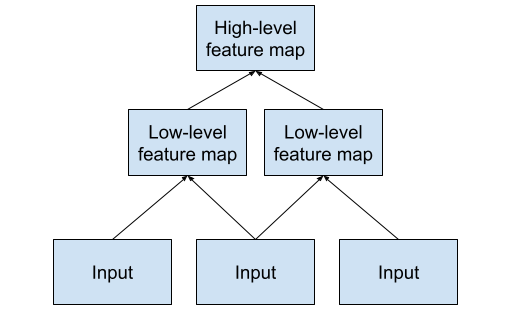
\includegraphics[width=1\linewidth]{resources/related_works/hierarchy.png}
        \caption{Classical Hierarchy}
        \label{fig:my_label}
    \end{subfigure}
    \hfill
    \begin{subfigure}[t]{0.3\textwidth}
        \centering
        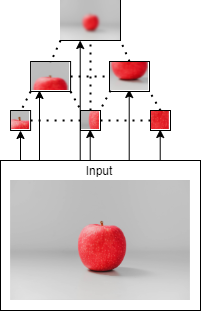
\includegraphics[width=1\linewidth]{resources/related_works/thousand_brains.png}
        \caption{Hierarchy as in the Thousand Brains Theory}
        \label{}
    \end{subfigure}
    \caption{Comparison of classical hierarchy and the hierarchy introduced by the Thousand Brains Theory}
\end{figure}
This new type of hierarchy is also quite similar to some state-of-the-art image recognition deep learning architectures such as InceptionNet\cite{inceptionnet} and Feature Pyramid Networks\cite{fpn}, in the sense that they apply different sized convolutional filters, where each filter can be thought of as its own separate model, on the data and do predictions based on all of them at once. This also ensures scale invariance of objects fed in to the architecture.
\begin{figure}[H]
    \centering
    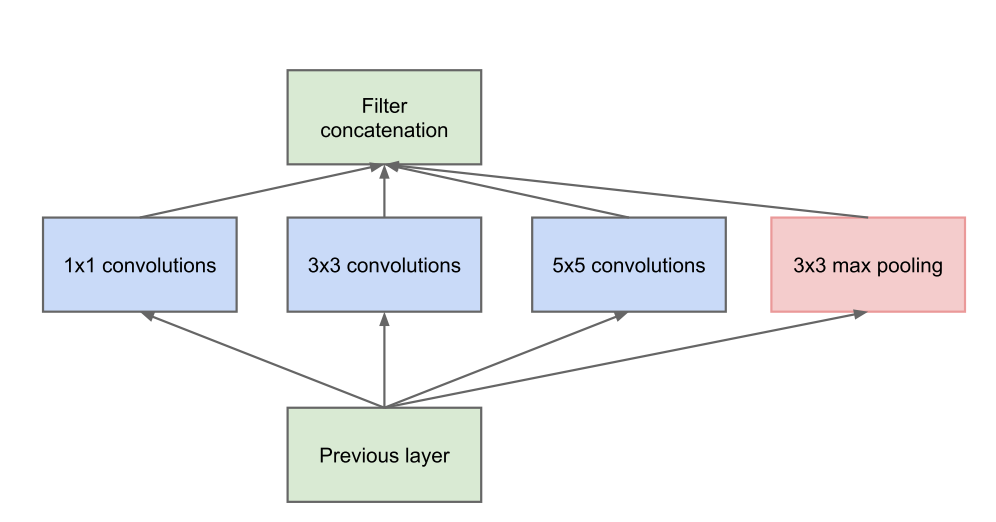
\includegraphics[width=\linewidth]{resources/models/inception_module.png}
    \caption{How the Inception \cite{inceptionnet} architecture combines multiple filters}
    \label{fig:inception_module}
\end{figure}

While the Thousand Brains Theory is not yet technically implemented in any way in a standard HTM model, it does show that recent developments within deep learning for image analysis have similarities with HTM theory.

\subsection{HTM Performance in Anomaly Detection}
\label{sec:htm_perf}
Knowing that deep learning approaches have a high degree of accuracy but suffer from problems related to generalizability, adaptability, and noise it stands to reason that HTM is a viable alternative for anomaly detection.\par
\cite{AHMAD2017134} explores the use of HTM for anomaly detection on low dimensional data such as temperature data from an industrial machine. The authors also discuss benchmarks for anomaly detection and compare different methods. The results show that HTM is very capable of performing anomaly detection, especially in a changing environment. HTM is able to outperform other anomaly detection methods and has the advantage of not requiring any per-problem parameter tuning.
\begin{figure}[H]
    \centering
    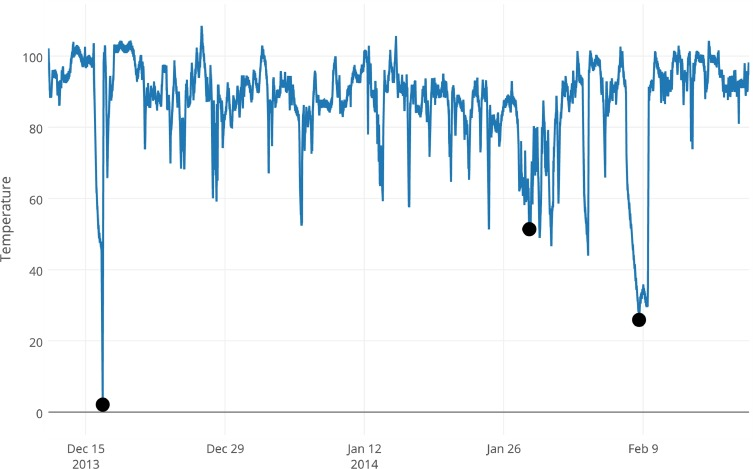
\includegraphics[width=0.75\linewidth]{resources/related_works/htm_anomaly_paper_example.jpg}
    \caption{Temperature anomaly detection from \cite{AHMAD2017134}.}
\end{figure}
For high-dimensional anomaly detection, \cite{MotionAnomalyDetection} used a HTM system to find anomalous frames in videos of motions. The anomalies were artificially created by swapping certain frames between different motion videos in the dataset. The results show that the HTM system was able to correctly detect some anomalies, but not an impressive amount. One thing to note is that direct binary representations of the video frames were used as SDRs, therefore no proper encoding was performed which might have led to the poor results. This hints at the fact that HTM by itself is not capable of handling high dimensional data, and is instead reliant on an encoder to lower the dimensionality by extracting important spatial features.
\begin{figure}[H]
    \centering
    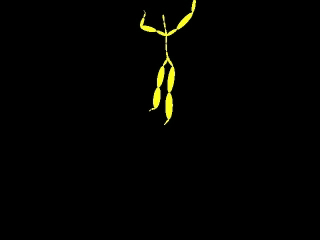
\includegraphics[width=0.5\linewidth]{resources/related_works/motion_frame.png}
    \caption{Example motion frame used in \cite{MotionAnomalyDetection}.}
\end{figure}
\subsection{Deep Learning HTM Encoder}
A potential solution to most of the aforementioned issues could be to combine the deep learning approaches with an HTM network. This way it could be possible to leverage the self-supervision and noise resilience property of HTM, together with the powerful feature extraction and representation of deep learning approaches. Effectively combining the best of both approaches while eliminating the disadvantages that have been previously mentioned.
\section{Summary}
\chapter{Grid HTM}
\label{sec:grid_htm}
\section{Introduction}
When it comes to applying \gls*{htm} on videos, this thesis proposes to use segmentation techniques to simplify the data into an SDR-friendly format. These segmentation techniques could be everything from simple binary thresholding to deep learning instance segmentation. Even keypoint detectors such as ORB\cite{orb_detector} could be applied. When explaining Grid HTM, the examples will be taken from deep learning instance segmentation of cars on a video from the VIRAT \cite{VIRAT} dataset.
\begin{figure}[H]
    \centering
    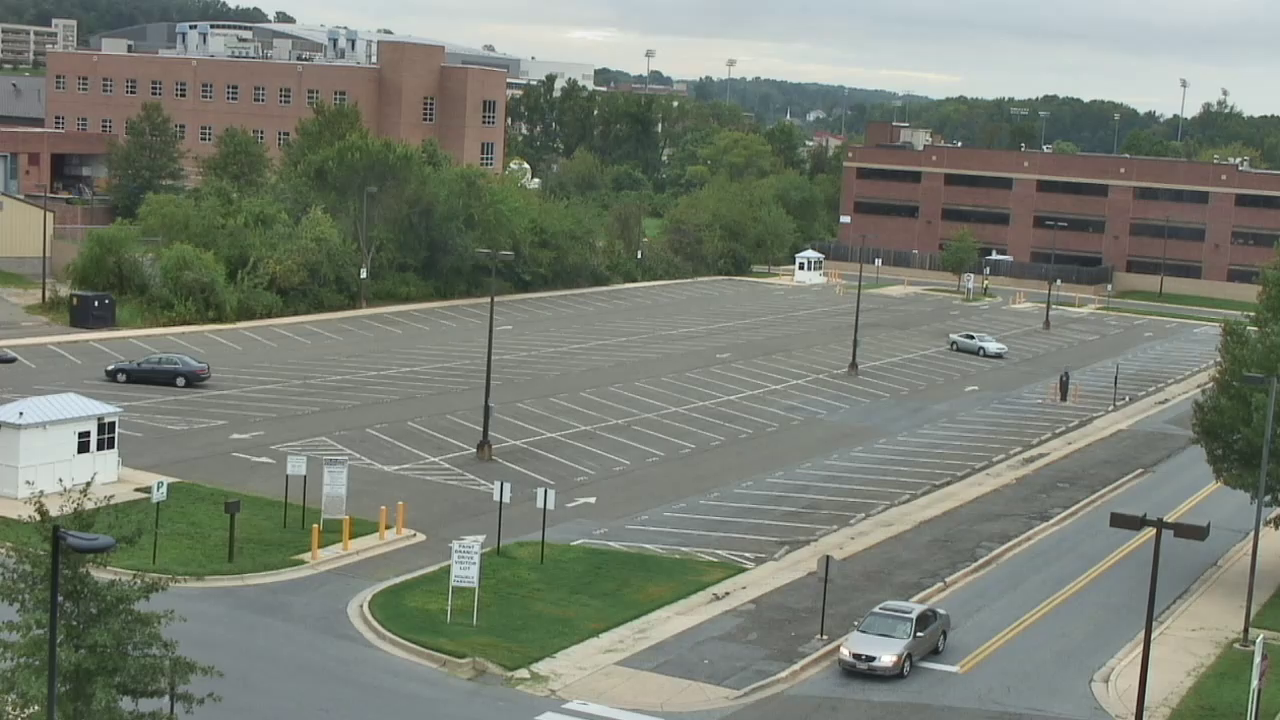
\includegraphics[width=.45\textwidth]{resources/methodology/original.png}
    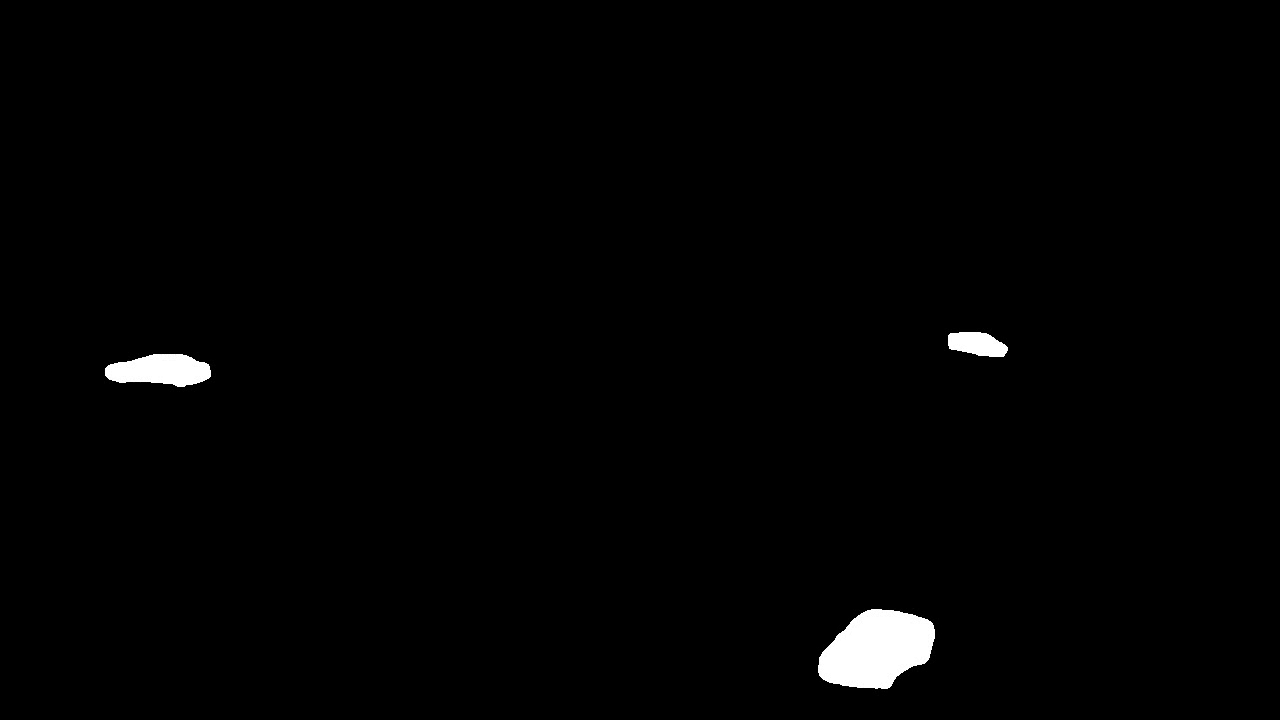
\includegraphics[width=.45\textwidth]{resources/methodology/car_segmentation.png}
    \caption{Segmentation result of cars, which is suited to be used as an SDR. Original frame taken from \cite{VIRAT}.}
\end{figure}
The idea is that the \gls*{sp} will learn to find an optimal general representation of cars. How general this representation is can be configured using the various parameters, but ideally they should be set so that different cars will be represented similarly while trucks and motorcycles will be represented differently.
\begin{figure}[H]
    \centering
    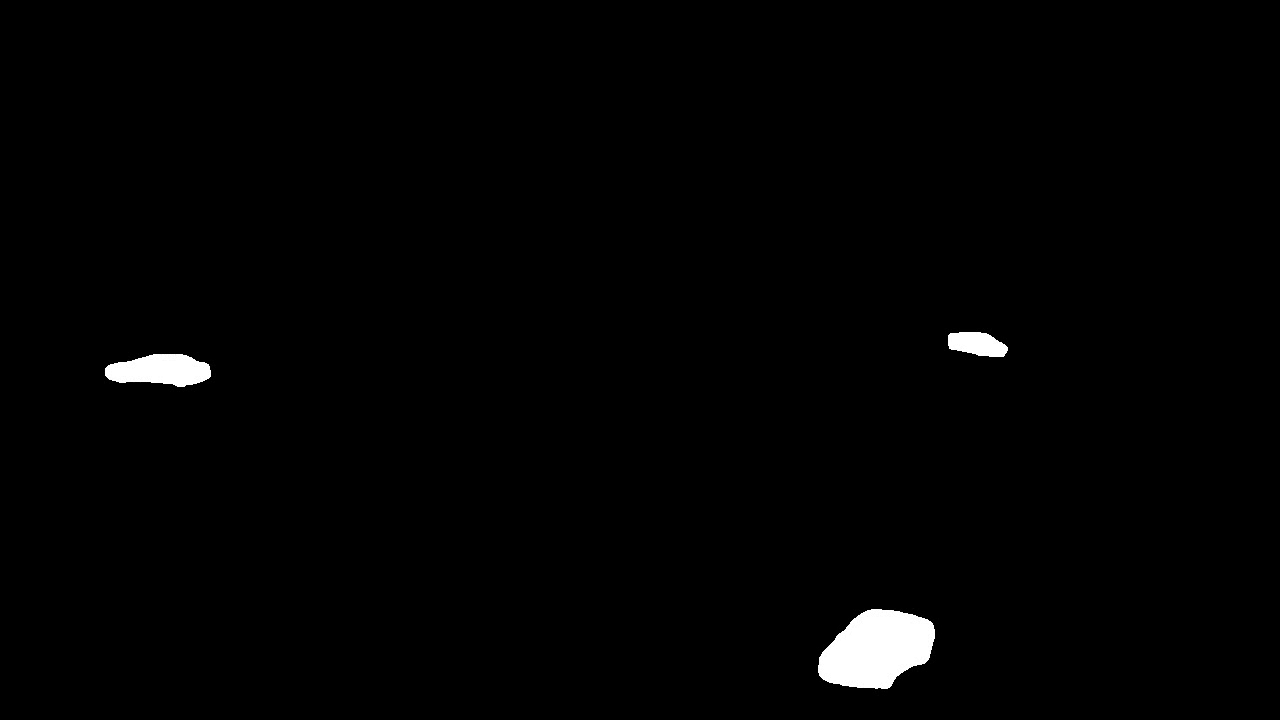
\includegraphics[width=.48\textwidth]{resources/methodology/car_segmentation.png}
    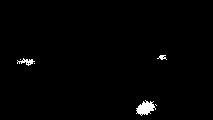
\includegraphics[width=.48\textwidth]{resources/methodology/car_segmentation_sp.png}
    \caption{The SDR and its corresponding \gls*{sp} representation. Note that the \gls*{sp} is untrained.}
\end{figure}
\par
The task of the \gls*{tm} will then be to learn the common patterns that the cars exhibit, their speed, shape, and positioning will be taken into account. Finally, the learning will be set so that new patterns are learned quickly, but forgotten slowly. This will allow the system to quickly learn the norm, even if there is little activity, while still reacting to anomalies. This requires that the input is stationary, in our example this means that the camera is not moving.
\par
Ideally, the system will have a calibration period spanning several days or weeks, during which the system is not performing any anomaly detection, but is just learning the patterns.\par
\section{Improvements}
\subsection{Invariance}
One issue that becomes evident is the lack of invariance. Because the \gls*{tm} is learning the global patterns, in our example it learns that it is normal for cars to drive along the road but only in the context of there being cars parked in the parking lot. It is instead desired that the \gls*{tm} learns that it is normal for cars to drive along the road, regardless of whether there are cars in the parking lot. This thesis proposes a solution based on dividing the encoder output into a grid, and have a separate \gls*{sp} and \gls*{tm} for each cell in the grid. The anomaly scores of all the cells are then aggregated into a single anomaly score using an aggregation function.
\begin{figure}[H]
    \centering
    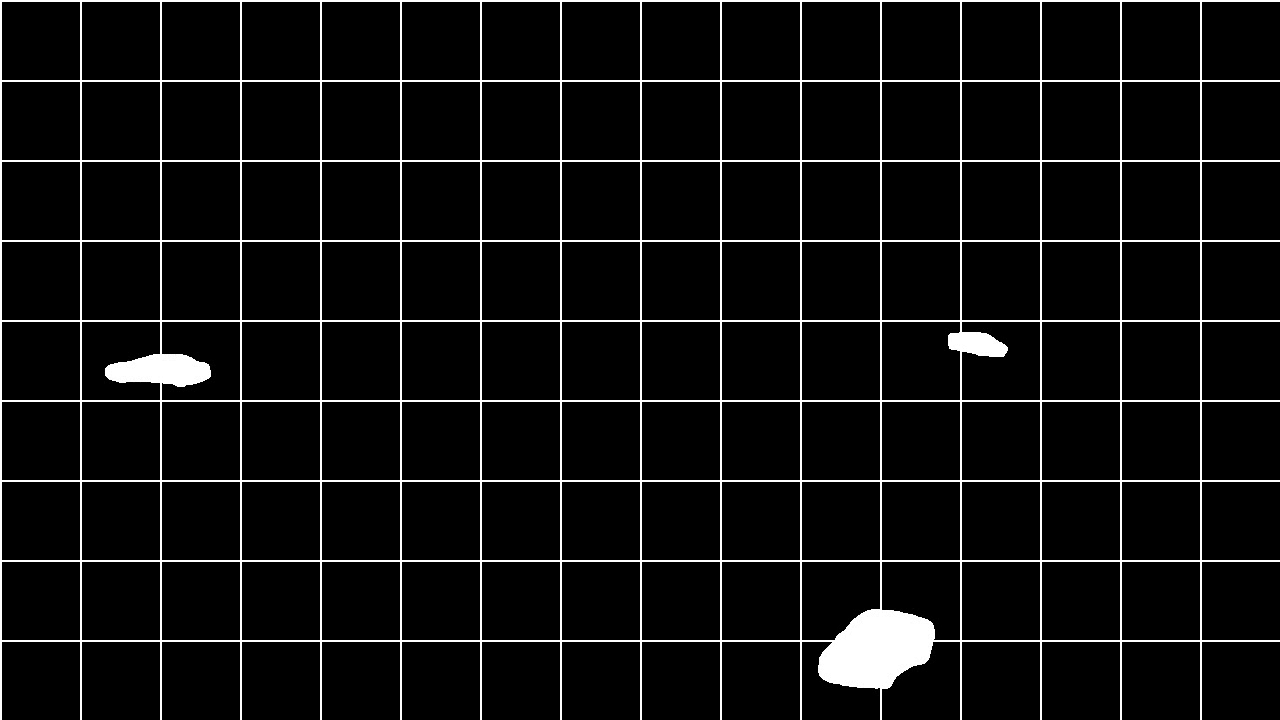
\includegraphics[width=\textwidth]{resources/methodology/car_segmentation_grid.png}
    \caption{The encoder output divided into a grid.}
    \label{fig:grid}
\end{figure}
\subsubsection{Aggregation Function}
Selecting the correct aggregation function is important because it affects the final anomaly output. For instance, it might be tempting to use the mean of all the anomaly scores as the aggregation function, but this leads to problems with normalization, meaning that an overall anomaly score of 1 is hard to achieve due to many cells having a zero anomaly score. In fact, it becomes unclear what a high anomaly score is anymore. Using the mean also means that anomalies that take up a lot of space will be weighted more than anomalies that take up a little space, which might not be desirable.

To solve the aforementioned problem and if the data has little noise, a potential aggregation function could be the non-zero mean:
\begin{align*}
    X         & :\{x : x > 0\} \\
    anomScore & =
    \begin{cases}
        \frac{\sum_{x \in X}x}{|X|} & \text{if } |X| > 0 \\
        0                           & \text{else}
    \end{cases}
\end{align*}
Meaning that only the cells with a non-zero anomaly score will be contributing to the overall anomaly score, which helps solve the aforementioned normalization and weighting problem. On the other hand, this will perform poorly when the system is exposed to noisy data which could lead to there always being one or more cells with a high anomaly score.
\begin{figure}[H]
    \centering
    \begin{subfigure}[t]{0.5\textwidth}
        \centering
        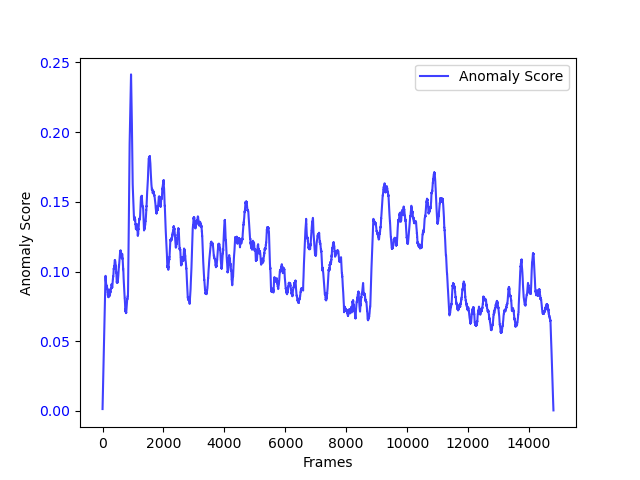
\includegraphics[width=\textwidth]{resources/methodology/aggr_noisy_mean.png}
        \caption{Mean.}
    \end{subfigure}%
    \begin{subfigure}[t]{0.5\textwidth}
        \centering
        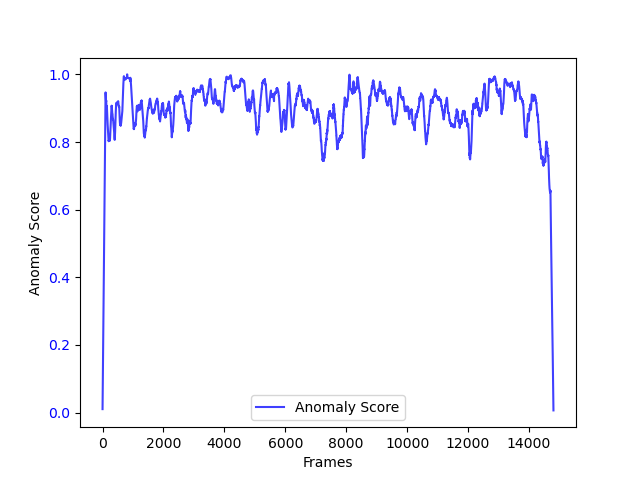
\includegraphics[width=\textwidth]{resources/methodology/aggr_noisy_nzmean.png}
        \caption{Non-zero mean.}
    \end{subfigure}
    \caption{How the two aggregation functions perform on the same noisy data.}
    \label{fig:aggr_noisy}
\end{figure}
\begin{figure}[H]
    \centering
    \begin{subfigure}[t]{0.5\textwidth}
        \centering
        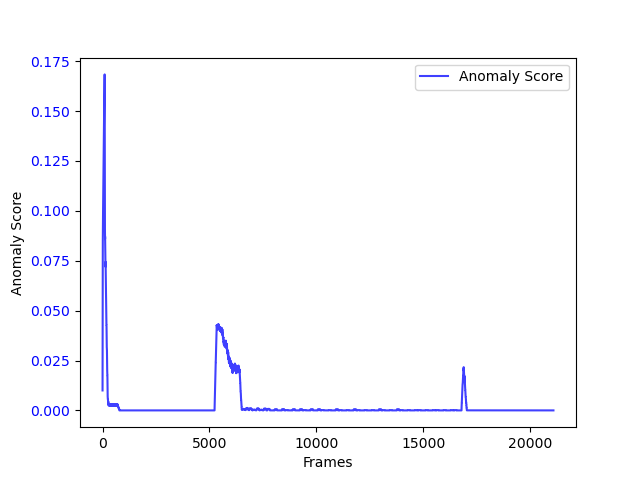
\includegraphics[width=\textwidth]{resources/methodology/aggr_clean_mean.png}
        \caption{Mean.}

    \end{subfigure}%
    \begin{subfigure}[t]{0.5\textwidth}
        \centering
        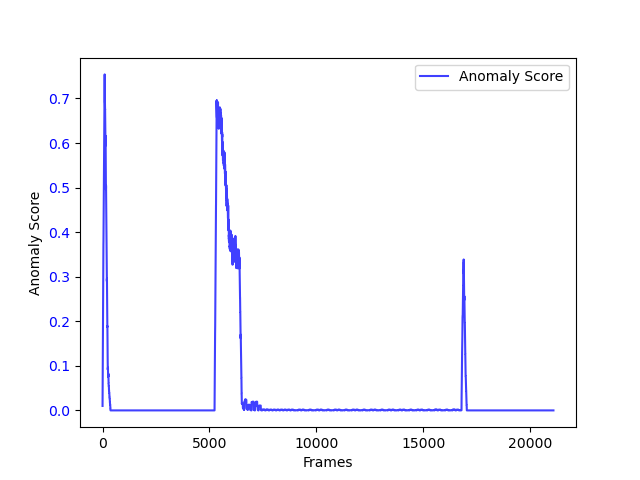
\includegraphics[width=\textwidth]{resources/methodology/aggr_clean_nzmean.png}
        \caption{Non-zero mean.}
    \end{subfigure}
    \caption{How the two aggregation functions perform on the same clean data.}
    \label{fig:aggr_clean}
\end{figure}
\autoref{fig:aggr_noisy} illustrates the effect of an aggregation function for noisy data, where the non-zero mean is rendered useless due to the noise. On the other hand, \autoref{fig:aggr_clean} shows how the non-zero mean gives a clearer anomaly score when the data is clean. Especially regarding how, unlike the mean, the non-zero mean has a clearly defined range between 0 and 1.
\subsection{Explainability}
Having the encoder output divided into a grid has the added benefit of introducing explainability into the model. By using Grid \gls*{htm} it is now possible to find out where in the input an anomaly has occurred. Combined with the ability to estimate the number of predictions at any given time for any cell, makes this an attractive approach.
\subsection{Flexibility and Performance}
In addition, it is also possible to configure the \gls*{sp} and the \gls*{tm} in each cell independently, giving the system increased flexibility. Last but not least, dividing the frame into smaller cells makes it possible to run each cell in parallel for increased performance.
\subsection{Reviewing Encoder Rules}
That being said, a potential problem with this approach is that the previously mentioned rules for creating a good encoder, see \autoref{sec:encoders}, may not be respected and therefore should be reviewed:
\begin{itemize}
    \item \textbf{Semantically similar data should result in SDRs with overlapping active bits}. In this example, a car at one position will produce an SDR with a high amount of overlapping bits as another car at a similar position in the input image.
    \item \textbf{The same input should always produce the same SDR}. The segmentation model produces a deterministic output given the same input.
    \item \textbf{The output must have the same dimensionality (total number of bits) for all inputs}. The segmentation model output has a fixed dimensionality.
    \item \textbf{The output should have similar sparsity (similar amount of one-bits) for all inputs and have enough one-bits to handle noise and subsampling}. The segmentation model does not respect this. An example is that there can be no cars (zero active bits), one car ($n$ active bits), or two cars ($2n$ active bits).
\end{itemize}
The solution for the last rule is two-fold, and  consists of imposing a soft upper bound and a soft lower bound for the number of active pixels within a cell. The purpose is to lower the variation of number of active pixels, while also containing enough semantic information for the \gls*{htm} to work:
\begin{itemize}
    \item Pick a cell size so that the distribution of number of active pixels is as tight as possible, while containing enough semantic information and also being small enough so that the desired invariance is achieved. The cell size acts as a soft upper bound for the possible number of active pixels.
    \item Create a pattern representing emptiness, where the number of active bits is similar to what can be expected on average when there are cars inside a cell. This acts as a soft lower bound for the number of active pixels.
\end{itemize}
There could be situations where a few pixels are active within a cell, which could happen when a car has just entered a cell, but this is fine as long as it does not affect the distribution too much. If it does affect the distribution, which can be the case with noisy data, then an improvement would be to add a minimum sparsity requirement before a cell is considered not empty, e.g. less than 5 active pixels means that the cell is empty.  In the following example, the number of active pixels within a cell centered in the video was used to build the distributions seen in \autoref{fig:num_active_pixels_dist}:
\begin{figure}[H]
    \centering
    \begin{subfigure}[t]{0.5\textwidth}
        \centering
        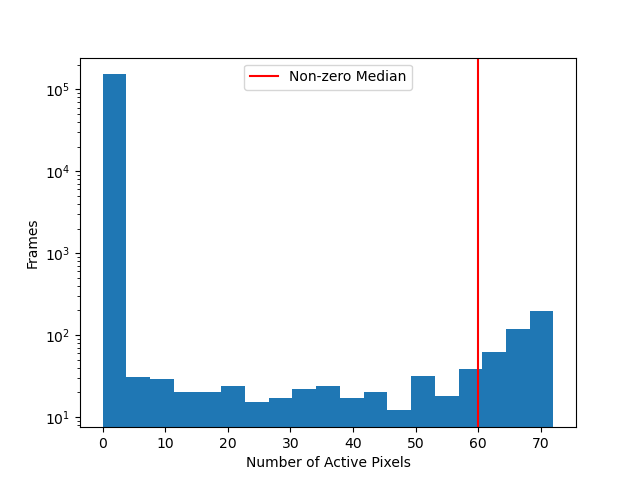
\includegraphics[width=\textwidth]{resources/methodology/active_pixels_dist.png}
        \caption{Without empty pattern.}
    \end{subfigure}%
    \begin{subfigure}[t]{0.5\textwidth}
        \centering
        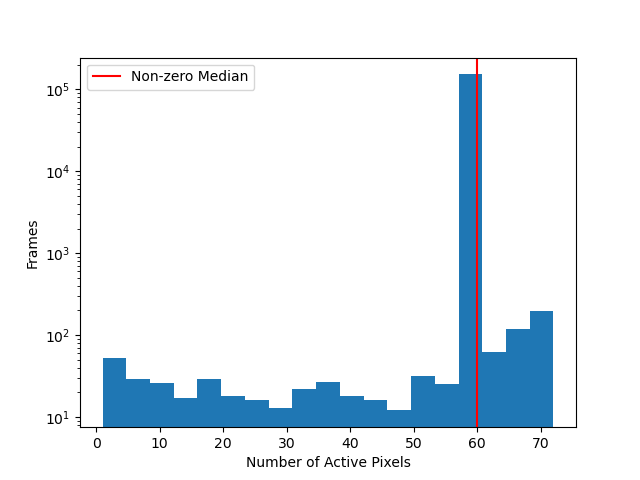
\includegraphics[width=\textwidth]{resources/methodology/active_pixels_dist2.png}
        \caption{With empty pattern.}
    \end{subfigure}
    \caption{Distribution of number of active pixels within a cell of size $12\times 12$, it can also be observed that it would benefit from having a minimum sparsity requirement of $\sim 5$.}
    \label{fig:num_active_pixels_dist}
\end{figure}


With a carefully selected empty pattern sparsity, \textbf{the standard deviation of active pixels was lowered from $\mathbf{3.78}$ to $\mathbf{1.88}$}. It is possible to automate this process by developing an algorithm which finds the optimal cell size and empty pattern sparsity which causes the least variation of number of active pixels per cell. This algorithm would run as a part of the calibration process.\par
The visual output resulting from these changes, which is an equally important output as the aggregated anomaly score, can be seen in \autoref{fig:gridhtm_output}:
\begin{figure}[H]
    \centering
    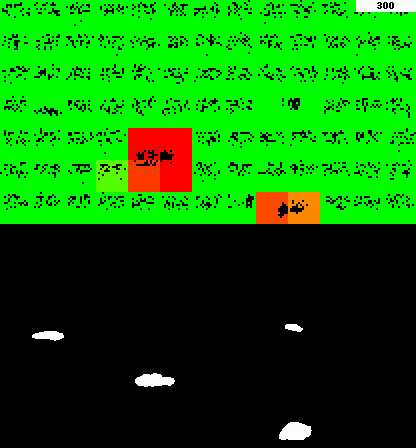
\includegraphics[width=0.7\textwidth]{resources/methodology/htm_grid_output.png}
    \caption{Example Grid \gls*{htm} output and the corresponding input. The color represents the anomaly score for each of the cells, where red means high anomaly score and green means zero anomaly score. Two of the cars are marked as anomalous because they are moving, which is something the Grid \gls*{htm} has not seen before during its 300 frame long lifetime.}
    \label{fig:gridhtm_output}
\end{figure}
Since there are now cells that are observing an empty pattern for a lot of the time in sparse data, boosting is recommended to be turned off, otherwise the \gls*{sp} output for the empty cells would change back and forth in order to adjust the active duty cycle.
\subsection{Stabilizing Anomaly Output}
\begin{figure}[H]
    \centering
    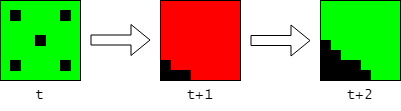
\includegraphics[width=0.7\textwidth]{resources/methodology/empty_to_notempty.png}
    \caption{High anomaly score when an empty cell (represented with an empty pattern with a sparsity value of 5) changes to being not empty, as something enters the cell.}
    \label{fig:empty_to_notempty}
\end{figure}
Another issue with the grid based approach is when a car first comes into a cell. The \gls*{tm} in that cell has no way of knowing that a car is about to enter, since it does not see outside its own cell, and therefore the first frame that a car enters a cell will cause a high anomaly output. This is illustrated in \autoref{fig:empty_to_notempty} where it can be observed that this effect causes the anomaly output to needlessly fluctuate. The band-aid solution is to ignore the anomaly score for the frame during which the cell goes from being empty to being not empty, which is illustrated in \autoref{fig:empty_to_notempty_fixed}.
\begin{figure}[H]
    \centering
    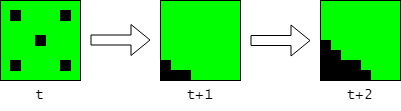
\includegraphics[width=0.7\textwidth]{resources/methodology/empty_to_notempty_fixed.png}
    \caption{In this case, the anomaly score is ignored (set to 0) for the frame in which the cell changes state from empty to not empty.}
    \label{fig:empty_to_notempty_fixed}
\end{figure}
A more proper solution could be to allow the \gls*{tm} to grow synapses to the TMs in the neighboring cells, but this is not documented in any research papers and might also hinder invariance.
\subsection{Multistep Temporal Patterns}
Since the \gls*{tm} can only grow segments to cells that were active in the previous timestep, as was mentioned in \autoref{sec:temporal_memory}, it will struggle to learn temporal patterns across multiple timesteps. This is especially evident in high framerate videos, where an object in motion has a similar representation at timestep $t$ and $t+1$, as an object standing still.
\begin{figure}[H]
    \centering
    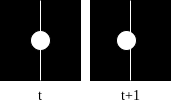
\includegraphics[width=0.3\textwidth]{resources/methodology/high_fps_moving.png}
    \unskip\ \vrule\
    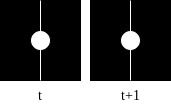
\includegraphics[width=0.3\textwidth]{resources/methodology/high_fps_still.png}
    \caption{Comparison of a moving object (left) and a still object (right)in a high framerate video. They are very similar and could actually end up being represented identically by the SP.}
\end{figure}
This could cause situations where an object that is supposed to be moving, suddenly stands still, yet the \gls*{tm} will not mark it as an anomaly due to it being stuck in a contextual loop. A contextual loop is when one of the predictions at $t$ becomes true at $t+1$, and then one of the predictions at $t+1$ is almost identical to the state at $t$, which becomes true if the object is not moving, causing the \gls*{tm} to enter the same state that it was in at $t$.
\begin{figure}[H]
    \centering
    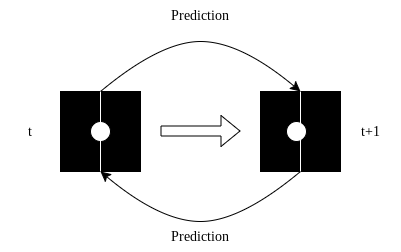
\includegraphics[width=0.7\textwidth]{resources/methodology/contextual_loop.png}
    \caption{Example of a contextual loop.}
\end{figure}
A solution is to concatenate the past $n$ \gls*{sp} outputs as input into the TM, which is made possible by keeping a buffer of past \gls*{sp} outputs and shifting its contents out as new \gls*{sp} outputs are inserted. This follows the core idea behind encoding time in addition to the data, which makes time act as a contextual anchor. However, in this case there are no timestamps that are suitable to be used as contextual anchors, so as a replacement, the past observations are encoded instead.
\par

\begin{figure}[H]
    \centering
    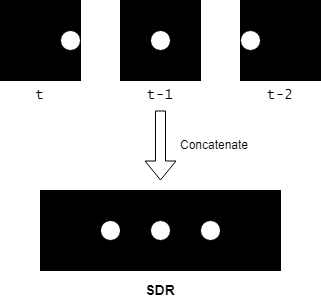
\includegraphics[width=0.45\textwidth]{resources/methodology/temporal_concatenation.png}
    \unskip\ \vrule\
    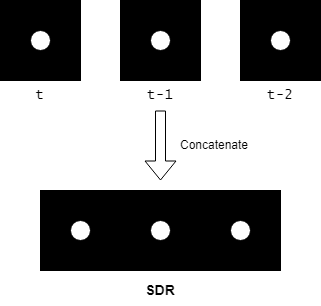
\includegraphics[width=0.45\textwidth]{resources/methodology/temporal_concatenation_still.png}
    \caption{Example of concatenation with $n=3$ when an object is moving from left to right, compared to when an object is not in motion. It can be observed that the SDRs are vastly different.}
\end{figure}
This will force the \gls*{tm} input, for when an object is in motion and when an object is still, to be unique. High framerate videos can benefit the most from this, and the effect will be more pronounced for higher values of $n$. One could feed the past $n$ encoder outputs into the \gls*{sp} instead, but this will lead to a much higher computational requirement, as well as make both the \gls*{sp} and \gls*{tm} parameters to be dependent on $n$.
\par
Adding support for multistep temporal patterns to the method used by \textcite{MotionAnomalyDetection}, which is mentioned in \autoref{sec:htm_perf}, could improve their results.
\section{Use Cases}
The most intuitive use case is to use Grid \gls*{htm} for semi-active surveillance, where personnel only have to look at segments containing anomalies, leading to drastically increased efficiency.
\par
One example is making it possible to have an entire city be monitored by a few people. This is made possible by making it so that people only have to look at segments that the Grid \gls*{htm} has found anomalous, which is what drastically lowers the manpower requirement for active monitoring of the entire city.
\par
Grid HTM could also be used to help automate labeling of anomaly datasets for deep learning. This would be similar to how older deep learning networks are used to help automate creating new labeled image datasets, where the model proposes a label for an image, which is then further refined by a human if needed.
\section{Summary}

\chapter{Experiments and Results}
\label{sec:experiments}
In this section, various experiments are performed in order to gauge the effectiveness of Grid HTM. There are three experiments in total, and each experiment covers a different use case. For the purpose of reproducibility, each experiment also includes tables showing the parameters used.
\section{Bouncing Ball Experiment}
To give credibility to the approach mentioned in \autoref{sec:grid_htm}, a simple experiment to test the capabilities of \gls*{htm} and confirm that they apply on a video is introduced.
\subsection{Data}
\begin{figure}[H]
    \centering
    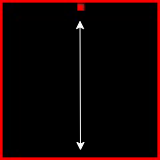
\includegraphics[width=.3\textwidth]{resources/experiments/bouncing_ball/bb_updown1.png}\hfill
    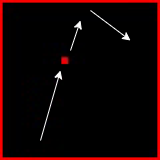
\includegraphics[width=.3\textwidth]{resources/experiments/bouncing_ball/bb_updownside.png}\hfill
    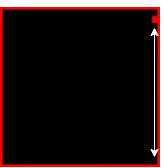
\includegraphics[width=.3\textwidth]{resources/experiments/bouncing_ball/bb_updown2.png}
    \caption[Bouncing Ball Experiment]{The bouncing ball experiment, and its three stages.}
    \label{fig:bb}
\end{figure}
The video consists of a ball bouncing up and down until an anomaly occurs in the form of a sudden introduction of a horizontal velocity. After a while this horizontal velocity is set back to 0 and the ball is once again bouncing up and down in-place. This is visualized in \autoref{fig:bb}.
\par
\subsection{HTM}
The model used is a standard \gls*{htm} model, which covers the entire input. This is equivalent to a single cell in a Grid HTM.
\begin{figure}[H]
    \centering
    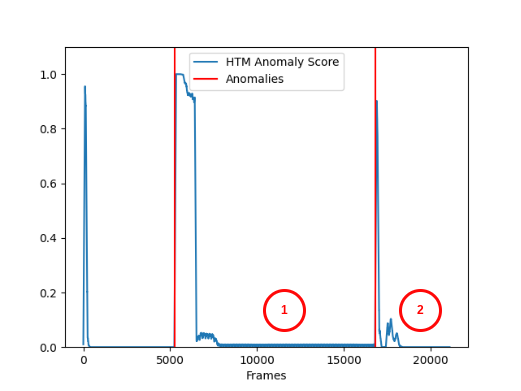
\includegraphics[width=0.9\textwidth]{resources/experiments/bouncing_ball/bb_anoms_bad.png}
    \caption[Bouncing Ball Experiment Anomaly Score]{The anomaly score in the bouncing ball experiment.}
    \label{fig:bb_normal}
\end{figure}
From \autoref{fig:bb_normal} it can be observed that \gls*{htm} correctly detects anomalies and quickly adapts to them. On the other hand, the result is not perfect due to the minor oscillations close to $(1)$ and the anomaly spikes towards the end close to $(2)$. While the imperfections are not major and can be safely ignored, it is still important to understand their causes and what can be done to improve upon them. \par
\subsubsection{Boosting}
The reason for the oscillations is due to the spatial pooler being dominated by a lucky few columns. The solution is to enable boosting, as explained in \autoref{sec:spatial_pooler}. This also helped with the spikes towards the end, as can be seen in \autoref{fig:bb_boosting}.\par
\begin{figure}[H]
    \centering
    \includegraphics[width=0.9\textwidth]{resources/experiments/bouncing_ball/bb_anoms_boosting.png}
    \caption[Bouncing Ball Experiment Anomaly Score No Boosting]{Bouncing ball with boosting enabled.}
    \label{fig:bb_boosting}
\end{figure}
\subsubsection{Zero Permanence Decrement}
The reason for the anomaly spikes towards the end is because the spatial pooler has found an optimal representation when the ball is bouncing freely, but when the ball stops and starts bouncing in-place the spatial pooler ends up unlearning the old optimal representation while it learns the new optimal representation. This causes a sudden minor change in the \gls*{sp} output, which the \gls*{tm} reports as anomalous.
\par
The solution is to set the value by which permanence is decreased by to zero, effectively disabling the ability of the spatial pooler to "forget", as can be seen in \autoref{fig:bb_forget}. That being said, the ability to decrement permanence is important in \gls*{htm} systems, therefore disabling it is not always feasible.
\begin{figure}[H]
    \centering
    \includegraphics[width=0.9\textwidth]{resources/experiments/bouncing_ball/bb_anoms_unforgetting.png}
    \caption[Bouncing Ball Experiment Anomaly Score Zero Decrement]{Bouncing ball without the ability of the \gls*{sp} to "forget".}
    \label{fig:bb_forget}
\end{figure}
\subsubsection{Boosting and Zero Permanence Decrement}
Finally, for the sake of interest, the bouncing ball example was performed with both boosting enabled and with zero permanence decrement. Results can be seen in \autoref{fig:bb_boosting_forget}.
\begin{figure}[H]
    \centering
    \includegraphics[width=0.9\textwidth]{resources/experiments/bouncing_ball/bb_anoms_unforgetting_boosting.png}
    \caption[Bouncing Ball Experiment Anomaly Score No Boosting Zero Decrement]{Bouncing ball without the ability of the \gls*{sp} to "forget" and with boosting enabled.}
    \label{fig:bb_boosting_forget}
\end{figure}
\subsubsection{Parameters}
Final list of parameters for reproducibility. For the plots, a moving average of $n=100$ was used to smooth the output. A lot of the parameters were selected through trial-and-error, and for most of the parameters, a change would lead to a minimal change in the results.
\begin{table}[H]
    \centering
    \begin{tabularx}{\linewidth}{@{}llX@{}}
        \toprule
        \textbf{Parameter} & \textbf{Value} & \textbf{Notes}                                                                       \\
        \midrule
        inputDimensions    & 120, 120       & The shape of the input                                                               \\
        columnDimensions   & 60, 60         & The dimensions of the columns in the spatial pooler                                  \\
        potentialPct       & 0.1            & Percent of inputs within the receptive field of a column that it can be connected to \\
        potentialRadius    & 120            & Controls the size of the receptive field                                             \\
        localAreaDensity   & 0.02           & Output SDR target sparsity                                                           \\
        globalInhibition   & True           & Set to False to enable topology                                                      \\
        wrapAround         & True           & Whether to wrap around the receptive field when it is outside the input SDR          \\
        synPermActiveInc   & 0.1            & Learning rate                                                                        \\
        synPermInactiveDec & 0              & Forgetting rate                                                                      \\
        stimulusThreshold  & 2              & Controls noise tolerance                                                             \\
        boostStrength      & 0.1            &                                                                                      \\
        dutyCyclePeriod    & 250            &                                                                                      \\
        seed               & 2              &                                                                                      \\
        \bottomrule
    \end{tabularx}

    \caption{SP Parameters}
    \label{tab:bb_sp_params}
\end{table}
\begin{table}[H]
    \centering
    \begin{tabularx}{\linewidth}{@{}llX@{}}
        \toprule
        \textbf{Parameter}        & \textbf{Value} & \textbf{Notes}                \\
        \midrule
        columnDimensions          & 60, 60         & Must be same as the \gls*{sp} \\
        predictedSegmentDecrement & 0.003          & Punishment forgetting rate    \\
        permanenceIncrement       & 0.1            & Learning rate                 \\
        permanenceDecrement       & 0.001          & Forgetting rate               \\
        minThreshold              & 3              & Controls noise tolerance      \\
        activationThreshold       & 5              & Controls noise tolerance      \\
        cellsPerColumn            & 16             & Contextual capacity           \\
        seed                      & 2              &                               \\
        \bottomrule
    \end{tabularx}

    \caption{TM Parameters}
    \label{tab:bb_TM_params}
\end{table}
\subsection{Grid HTM}
This is a very simple problem which does not require invariances, making it unsuitable for Grid HTM. Grid \gls*{htm} would be suitable if there were two or more independent bouncing balls, due to its improved invariance. Still, it is interesting to see how Grid \gls*{htm} performs compared to normal HTM.
\subsubsection{Results}
\begin{figure}[H]
    \centering
    \includegraphics[width=0.9\textwidth]{resources/experiments/bouncing_ball/bb_grid}
    \caption[Bouncing Ball Experiment Anomaly Score Grid HTM]{Results when using Grid HTM}
    \label{fig:bb_gridhtm}
\end{figure}
It can be observed in \autoref{fig:bb_gridhtm} that Grid \gls*{htm} performs worse than the normal HTM, due to the more prominent anomaly score spikes seen in \autoref{fig:bb_boosting_forget}, but the result is still acceptable. This is to be expected since this problem is not suited for Grid HTM, and that the parameters given in \autoref{tab:bb_gridhtm_params}, \autoref{tab:bb_sp_gridhtm_param}, and \autoref{tab:bb_tm_gridhtm_param} are probably not optimal.
\subsubsection{Parameters}
The \gls*{sp} and \gls*{tm} parameters were selected so that they were as close as possible to the normal \gls*{htm} parameters. The non-zero mean was chosen as the aggregation function, because there is no noise due to the controlled environment. Again, a moving average of $n=100$ was used to smooth the anomaly score output in the plots. A lot of the parameters were selected through trial-and-error, and for most of the parameters, a change would lead to a minimal change in the results.
\begin{table}[H]
    \centering
    \begin{tabularx}{\linewidth}{@{}XlX@{}}
        \toprule
        \textbf{Parameter} & \textbf{Value} & \textbf{Notes}                                                                                                          \\
        \midrule
        sp\_grid\_size     & (30, 30)       & Size of each cell in the grid, affects invariance                                                                       \\
        tm\_grid\_size     & (15, 15)       & Dimension of the \gls*{sdr} that each \gls*{sp}    outputs, also the number of columns in the \gls*{sp}                 \\
        min\_sparsity      & 1              & How many pixels for the grid cell to be considered not empty, here it is set to mimic normal HTM                        \\
        sparsity           & 28.27          & Empty pattern active bits, here it is the area of the bouncing ball with $r=3$                                          \\
        temporal\_size     & 1              & Size of the multistep temporal pattern, 1 means it is effectively disabled, it is disabled in order to mimic normal HTM \\
        \bottomrule
    \end{tabularx}
    \caption{Grid HTM specific parameters}
    \label{tab:bb_gridhtm_params}
\end{table}
\begin{table}[H]
    \centering
    \begin{tabularx}{\linewidth}{@{}XlX@{}}
        \toprule
        \textbf{Parameter} & \textbf{Value} & \textbf{Notes}                                                                                                                                        \\
        \midrule
        inputDimensions    & sp\_grid\_size &                                                                                                                                                       \\
        columnDimensions   & tm\_grid\_size &                                                                                                                                                       \\
        potentialPct       & 0.5            & Percent of inputs within the receptive field of a column that it can be connected to, increased in order to compensate for the smaller potential pool \\
        potentialRadius    & 5              & Controls the size of the receptive field                                                                                                              \\
        localAreaDensity   & 0.1            & Output SDR target sparsity                                                                                                                            \\
        globalInhibition   & True           & Set to False to enable topology                                                                                                                       \\
        wrapAround         & False          & Whether to wrap around the receptive field when it is outside the input SDR                                                                           \\
        synPermActiveInc   & 0.1            & Learning rate                                                                                                                                         \\
        synPermInactiveDec & 0.001          & Forgetting rate                                                                                                                                       \\
        stimulusThreshold  & 2              & Controls noise tolerance                                                                                                                              \\
        boostStrength      & 0              & Set to 0 to avoid instability in empty cells                                                                                                          \\
        seed               & 2              &                                                                                                                                                       \\
        \bottomrule
    \end{tabularx}
    \caption{SP Parameters}
    \label{tab:bb_sp_gridhtm_param}
\end{table}
\begin{table}[H]
    \centering
    \begin{tabularx}{\linewidth}{@{}XlX@{}}
        \toprule
        \textbf{Parameter}        & \textbf{Value} & \textbf{Notes}             \\
        \midrule
        columnDimensions          & tm\_grid\_size & Same as the \gls*{sp}      \\
        predictedSegmentDecrement & 0.003          & Punishment forgetting rate \\
        permanenceIncrement       & 0.1            & Learning rate              \\
        permanenceDecrement       & 0.001          & Forgetting rate            \\
        minThreshold              & 1              & Controls noise tolerance   \\
        activationThreshold       & 1              & Controls noise tolerance   \\
        cellsPerColumn            & 16             & Contextual capacity        \\
        seed                      & 2              &                            \\
        \bottomrule
    \end{tabularx}
    \caption{TM Parameters}
    \label{tab:bb_tm_gridhtm_param}
\end{table}
\subsection{Experiment Summary}
This experiment is a controlled experiment involving a computer generated ball bouncing up and down, and then introducing an anomaly in the form of a change in horizontal velocity. Finally, the horizontal velocity is set back to zero.
\par
First the experiment is performed with a normal \gls*{htm} model, and the results show that it is capable of detecting the anomalies and quickly adapts to them. The same experiment is then performed with Grid HTM. The results show that Grid \gls*{htm} is also capable of detecting the anomalies and quickly adapts to them, however it performs slightly worse than normal HTM. The reason is that Grid \gls*{htm} is designed for more complex videos, such as if there were multiple bouncing balls at once.
\clearpage
\section{Surveillance Experiment}
As stated earlier, one of the use cases of Grid \gls*{htm} is anomaly detection in complex videos. This example will show how Grid \gls*{htm} could perform on surveillance footage.
The video to be used is part of the VIRAT~\cite{VIRAT} video dataset, and was selected due to its long duration and stationary camera, which is shown in \autoref{fig:selected_frame}.
\par
The downside is that the video does not contain any non-technical anomalies, but consists of technical anomalies in the form of several segments with sudden frame skips in between. There is also a synthetic anomaly introduced in the form of a frame repeat lasting a couple of seconds, essentially "freezing" time, in order to test whether Grid \gls*{htm} is able to understand how objects should be moving in time.
\begin{figure}[H]
    \centering
    \includegraphics[width=0.8\textwidth]{resources/methodology/original.png}
    \includegraphics[width=0.8\textwidth]{resources/experiments/surveillance/parking_frame.png}
    \caption[Example Frames]{Example frames from the selected video.}
    \label{fig:selected_frame}
\end{figure}
As previously mentioned, both binary thresholding and deep learning feature map extraction as encoders have their downsides. Therefore, this thesis proposes to use a combination of both, a segmentation model which can extract classes into their respective SDRs. Meaning that there could be a \gls*{sdr} for cars and a \gls*{sdr} for persons (see \autoref{fig:seg_car_person}), that are then concatenated before being fed into the system.
\par
The segmentation model used is PointRend~\cite{pointrend} with a ResNet101~\cite{resnet} backbone, pretrained on ImageNet~\cite{imagenet}, and implemented using PixelLib~\cite{pixellib}.
\begin{figure}[H]
    \centering
    \includegraphics[width=0.45\textwidth]{resources/methodology/car_segmentation.png}
    \includegraphics[width=0.45\textwidth]{resources/methodology/person_segmentation.png}
    \caption[Example Segmentation of Cars and Persons]{Example segmentation of cars and persons.}
    \label{fig:seg_car_person}
\end{figure}
For the sake of simplicity, this experiment will focus only on the segmentation of cars.
\par
While on the topic of segmentation, it is important to mention that the segmentation model is not perfect and that there are cases where objects are misclassified as well as cases where cars repeatedly go above and below the confidence threshold.
\subsection{Results}
\begin{figure}[H]
    \centering
    \includegraphics[width=\textwidth]{resources/experiments/surveillance/surveillance_result}
    \caption[Grid HTM Anomaly Score Output]{Anomaly score output from Grid HTM.}
    \label{fig:surveillance_results}
\end{figure}
It can be observed in \autoref{fig:surveillance_results} that Grid \gls*{htm} is detecting when segments begin and end, however it is not possible to use a threshold value to isolate them, and they also have vastly different anomaly scores compared to each other. This is due to the way the aggregation function works, which means that the anomaly output is dependent on the physical size of the anomaly. It should also be noted that a moving average ($n=200$) was applied to smooth out the anomaly score output, otherwise the graph would be too noisy.
\par
With the aggregation functions presented in this thesis in mind, it is safe to conclude that looking at the anomaly score output is meaningless for complex data such as a surveillance video. This however does not mean that Grid \gls*{htm} is completely useless, and this can be observed by looking at the visual output of Grid HTM. The visual output during which the first segment anomaly occurs can be seen in \autoref{fig:surveillance_segment}.
\begin{figure}[H]
    \centering
    \includegraphics[width=\textwidth]{resources/experiments/surveillance/surveillance_anomaly_1.png}
    \caption[Segment Anomaly]{The first segment anomaly, which is marked with red text,  and the corresponding changes detected by Grid HTM.}
    \label{fig:surveillance_segment}
\end{figure}
Here it is observed that Grid \gls*{htm} correctly marks the sudden change of cars when the current segment ends and a new segment begins.
\subsubsection{Road}
In the original video, there is a road on which cars regularly drive. By observing the visual output, it becomes evident that after some time, Grid \gls*{htm} has mostly learned that behavior and does not report those moving cars as anomalies. This is shown in \autoref{fig:surveillance_road_1}.
\begin{figure}[H]
    \centering
    \includegraphics[width=\textwidth]{resources/experiments/surveillance/surveillance_road_1.png}
    \caption[Car Driving Along Main Road]{Visual output during when a car is driving along the main road.}
    \label{fig:surveillance_road_1}
\end{figure}
\subsubsection{Frame Repeat}
To prove that Grid \gls*{htm} has learned that cars on the road should be moving, it is possible to look at the visual output during the period when the video is repeating the same frame and observe if the architecture marks the cars standing still on the road as anomalies.
\begin{figure}[H]
    \centering
    \includegraphics[width=\textwidth]{resources/experiments/surveillance/surveillance_freeze_1.png}
    \caption[Frame Repeat Anomaly]{Anomaly output during the repeating frame, the start of the frame repeat is marked with red text. The blue circle highlights the object of interest.}
    \label{fig:surveillance_freeze_1}
\end{figure}
It can be observed in \autoref{fig:surveillance_freeze_1} that the cars along the main road are not marked as anomalies, but this could be attributed to the fact that there is a crossing there and that cars periodically have to stop at that point to let pedestrians cross.
\par
On the other hand, when looking at the anomaly marked with a blue circle, the car on the road in the parking lot is marked as an anomaly that increases in severity as the time goes on during the frame repeat. The reason why that car causes an anomaly is because, unlike the cars on the main road, a car is rarely observed as standing still at that position.
\par
To prove that the anomaly was actually directly caused by the repeating frame, and not just due to repeating the anomaly in time, it should be compared to the anomaly output if there was no repeating frame.
\begin{figure}[H]
    \centering
    \includegraphics[width=\textwidth]{resources/experiments/surveillance/surveillance_freeze_no_freeze.png}
    \caption[No Frame Repeat Anomaly]{Anomaly output when there is no frame repeating, where it should have repeated is marked in red. The blue circle highlights the object of interest.}
    \label{fig:surveillance_freeze_no_freeze}
\end{figure}
It can be observed in \autoref{fig:surveillance_freeze_no_freeze} that the anomaly output is minor compared to when there was a repeating frame, proving that the anomaly was indeed a product of the repeating frame and that Grid \gls*{htm} was able to learn how objects should be moving in time.
\par
Finally, it is interesting to look at how Grid \gls*{htm} handles the repeating frames without multistep temporal patterns, which is shown in \autoref{fig:surveillance_freeze_no_mtp}.
\begin{figure}[H]
    \centering
    \includegraphics[width=\textwidth]{resources/experiments/surveillance/surveillance_freeze_no_mtp.png}
    \caption[Frame Repeat No Multistep Temporal Pattern Anomaly]{Anomaly output during the repeating frame, the start of the frame repeat is marked with red text. The blue circle highlights the object of interest. This time without multistep temporal patterns.}
    \label{fig:surveillance_freeze_no_mtp}
\end{figure}
Unfortunately, simply disabling multistep temporal patterns without adjusting the other \gls*{tm} parameters causes the same car to be marked as an anomaly before and during the frame repeat. In fact, as mentioned in \autoref{sec:multistep_temporal_patterns}, disabling multistep temporal patterns causes Grid \gls*{htm} to be less noise tolerant which causes a lot more anomalies to be wrongly detected. This is evident in \autoref{fig:surveillance_freeze_no_mtp}, where a higher number of severe anomalies can be observed compared to previous examples. This also highlights how sensitive \gls*{htm} can be regarding parameters.
\subsubsection{Points of Interest}
Finally, it is interesting to look the various anomaly score spikes and observe in the visual output what caused them. The points of interest to be explored are marked in \autoref{fig:surveillance_poi}
\begin{figure}[H]
    \centering
    \includegraphics[width=\textwidth]{resources/experiments/surveillance/surveillance_result_poi.eps}
    \caption[Points of Interest]{Points of interests in the anomaly score output.}
    \label{fig:surveillance_poi}
\end{figure}
The first point of interest, which can be seen in \autoref{fig:surveillance_poi_1}, showcases the weakness of the aggregation function.
\begin{figure}[H]
    \centering
    \includegraphics[width=\textwidth]{resources/experiments/surveillance/surveillance_poi_1.png}
    \caption[First POI]{Visual output of the first point of interest.}
    \label{fig:surveillance_poi_1}
\end{figure}
It can be seen that the anomaly score output, which is shown at the very bottom of each image, can be attributed to two occurrences. The first occurrence is a physically big but low severity anomaly. The second occurrence is a physically small but high severity anomaly. Despite the two different anomalies, the anomaly score output is similar for both occurrences.
\par
The second point of interest, which can be seen in \autoref{fig:surveillance_poi_2}, showcases the importance of exposing \gls*{htm} to all possible behaviors that are considered not anomalous, which is one of the complexities mentioned in \autoref{sec:anomaly_detection}.
\begin{figure}[H]
    \centering
    \includegraphics[width=\textwidth]{resources/experiments/surveillance/surveillance_poi_2.png}
    \caption[Second POI]{Visual output of the second point of interest.}
    \label{fig:surveillance_poi_2}
\end{figure}
It can be observed that there are high anomaly outputs for cars entering the parking lot from the left side of the frame. The high anomaly score is caused by an insufficient number of previous observations of that behavior.
\subsection{Parameters}
Final list of parameters for reproducibility. As previously mentioned, a moving average ($n=200$) was used to smooth the output graph and make it more readable. The mean was used as the aggregation function due to the complex nature of the data. Most of the parameters were selected through trial-and-error and are also exaggerated in order to compensate for the relatively short video duration compared to what Grid HTM is designed for.
\begin{table}[H]
    \centering
    \begin{tabularx}{\linewidth}{@{}XlX@{}}
        \toprule
        \textbf{Parameter} & \textbf{Value} & \textbf{Notes}                                                                  \\
        \midrule
        sp\_grid\_size     & (32, 32)       & Size of each cell in the grid, affects invariance                               \\
        tm\_grid\_size     & (16, 16)       & Dimension of the SDR that each SP outputs, also the number of columns in the SP \\
        min\_sparsity      & 10             & How many pixels for the grid cell to be considered not empty                    \\
        sparsity           & 15             & Empty pattern active bits                                                       \\
        temporal\_size     & 15             & Size of the multistep temporal pattern buffer                                   \\
        \bottomrule
    \end{tabularx}
    \caption{Grid HTM specific parameters}
    \label{tab:surveillance_grid_htm}
\end{table}
\begin{table}[H]
    \centering
    \begin{tabularx}{\linewidth}{@{}XlX@{}}
        \toprule
        \textbf{Parameter} & \textbf{Value} & \textbf{Notes}                                                                       \\
        \midrule
        inputDimensions    & sp\_grid\_size &                                                                                      \\
        columnDimensions   & tm\_grid\_size &                                                                                      \\
        potentialPct       & 0.2            & Percent of inputs within the receptive field of a column that it can be connected to \\
        potentialRadius    & 5              & Controls size of the receptive field                                                 \\
        localAreaDensity   & 0.05           & Output SDR target sparsity                                                           \\
        globalInhibition   & True           & Set to False to enable topology                                                      \\
        wrapAround         & False          & Whether to wrap around the receptive field when it is outside the input \gls*{sdr}   \\
        synPermActiveInc   & 0.01           & Learning rate                                                                        \\
        synPermInactiveDec & 0.00001        & Forgetting rate                                                                      \\
        stimulusThreshold  & 3              & Controls noise tolerance                                                             \\
        boostStrength      & 0              & Causes instability in empty cells                                                    \\
        seed               & 2              &                                                                                      \\
        \bottomrule
    \end{tabularx}
    \caption{SP Parameters}
    \label{tab:surveillance_sp}
\end{table}
\begin{table}[H]
    \centering
    \begin{tabularx}{\linewidth}{@{}XlX@{}}
        \toprule
        \textbf{Parameter}        & \textbf{Value} & \textbf{Notes}             \\
        \midrule
        columnDimensions          & tm\_grid\_size & Same as the \gls*{sp}      \\
        predictedSegmentDecrement & 0.001          & Punishment forgetting rate \\
        permanenceIncrement       & 0.01           & Learning rate              \\
        permanenceDecrement       & 0.001          & Forgetting rate            \\
        minThreshold              & 10             & Controls noise tolerance   \\
        activationThreshold       & 10             & Controls noise tolerance   \\
        cellsPerColumn            & 32             & Contextual capacity        \\
        seed                      & 2              &                            \\
        \bottomrule
    \end{tabularx}
    \caption{TM Parameters}
    \label{tab:surveillance_tm}
\end{table}
\subsection{Experiment Summary}
This experiment showcases the performance of Grid \gls*{htm} on complex data, specifically a surveillance video of a parking lot. The video contains technical anomalies in the form of segments, and also a synthetic anomaly which is a period of repeating frames. Semantic segmentation was performed in order to extract the cars in the frame into an SDR.
\par
The results show that Grid \gls*{htm} has the ability to react when segments begin and end, as well as the ability to detect the repeating frames. It also shows that the anomaly output, with the currently introduced aggregation functions, cannot be used to reliably to threshold anomalies. Instead, one can look at the visual output of Grid HTM. The visual output shows that Grid \gls*{htm} is able to detect the change in objects when a segment change occurs.
\par
Results also show that Grid \gls*{htm} learns common patterns such as cars driving on the main road, and does not report that behavior as anomalous. It is also shown that Grid \gls*{htm} can correctly detect the repeating frames, and marks anomalous cars during the repeating frames with an increasing severity. Finally, a couple of points of interests are shown that highlight the weakness of the aggregation function and the importance of exposing \gls*{htm} to all possible behaviors not considered anomalous.
\clearpage
\section{Sperm Experiment}
As seen in the surveillance experiment, it seems Grid \gls*{htm} can detect when segments begin and end. This experiment will explore this ability in greater detail.
\subsection{Data}
The dataset used is VISEM~\cite{VISEM}, a sperm dataset which consists of videos that are made up of several segments. The sperm cells will be segmented using a rough binary thresholding, as shown in \autoref{fig:sperm_segmentation}.
\begin{figure}[H]
    \centering
    \includegraphics[width=.45\textwidth]{resources/experiments/sperm/sperm_example.png}
    \includegraphics[width=.45\textwidth]{resources/experiments/sperm/sperm_seg_example.png}
    \caption[Sperm Example Frame]{Example frame from a sperm video (left) and its corresponding segmentation (right).}
    \label{fig:sperm_segmentation}
\end{figure}
It is important to note that the data itself is noisy, and that it is not possible for Grid \gls*{htm} to learn any meaningful patterns. The individual videos are also relatively short, which makes it even harder to learn any meaningful patterns.
\subsection{Benchmark}
To ensure that \gls*{htm} does not just react to the sudden change in pixels but does something more, the L1 error will be used as a benchmark to compare against:
\begin{align*}
    E_t=\sum|F_t-F_{t-1}|
\end{align*}
Where $F_t$ denotes a segmented frame at time step $t$. The L2 error could also have been used, but it would not matter since this experiment will be comparing relative values.
\subsection{Results}
As seen in \autoref{fig:sperm_results1}, Grid \gls*{htm} is able to outperform the L1 error benchmark. This can be deduced from the more prominent changes in the anomaly score, compared to the L1 error. The reason might be that even though the data is very noisy, there is still something in it which makes Grid \gls*{htm} able to learn something general about the current state. This could for instance be a single cell that is standing still or moving very slowly, which Grid \gls*{htm} anchors itself to and uses it to determine when segments start and end.
\begin{figure}[H]
    \centering
    \includegraphics[width=\textwidth]{resources/experiments/sperm/sperm_result1.png}
    \caption[Stationary Video Results]{Results on a stationary sperm video.}
    \label{fig:sperm_results1}
\end{figure}

\par
That being said, the parameters for Grid \gls*{htm} were selected carefully to achieve the results seen in \autoref{fig:sperm_results1}, and are dependent on the contents of the data. Unfortunately, most of the videos in the dataset contain drift (in other words, the video is not stationary), which makes Grid \gls*{htm} useless. This can be observed in \autoref{fig:sperm_results2}, where both Grid \gls*{htm} and the L1 error struggle.
\begin{figure}[htb]
    \centering
    \includegraphics[width=\textwidth]{resources/experiments/sperm/sperm_result2.png}
    \caption[Drifting Video Results]{Results on a sperm video with drift.}
    \label{fig:sperm_results2}
\end{figure}
Just like in the stationary video, the change in the anomaly score is more pronounced, but due to the drift in the video there is a constant high anomaly output which makes it impossible to find a threshold value. That being said, Grid \gls*{htm} still outperforms the L1 score due to the more prominent changes in the anomaly score.
\subsection{Use Cases}
The use case is to be able to use Grid \gls*{htm} to detect segments and then use a separate tool to extract each segment. This could be useful in data processing, or even in streaming media services to automatically know when cuts happen and could aid scene boundary detection systems~\cite{scene_boundary_detection}.
\subsection{Parameters}
The following parameters were used in this experiment. The main difference from the surveillance experiment to note is the temporal size, which has been disabled due to the nonexistent patterns in the data. Again, the parameters were mostly selected through an educated trial-and-error method.
\begin{table}[H]
    \centering
    \begin{tabularx}{\linewidth}{@{}XlX@{}}
        \toprule
        \textbf{Parameter} & \textbf{Value} & \textbf{Notes}                                                                  \\
        \midrule
        sp\_grid\_size     & (16, 16)       & Size of each cell in the grid, affects invariance                               \\
        tm\_grid\_size     & (8, 8)         & Dimension of the SDR that each SP outputs, also the number of columns in the SP \\
        min\_sparsity      & 1              & How many pixels for the grid cell to be considered not empty                    \\
        sparsity           & 5              & Empty pattern active bits                                                       \\
        temporal\_size     & 1              & Size of the multistep temporal pattern buffer                                   \\
        seed               & 2              &                                                                                 \\
        \bottomrule
    \end{tabularx}
    \caption{Grid HTM specific parameters}
    \label{tab:sperm_params}
\end{table}
\begin{table}[H]
    \centering
    \begin{tabularx}{\linewidth}{@{}XlX@{}}
        \toprule
        \textbf{Parameter} & \textbf{Value} & \textbf{Notes}                                                                       \\
        \midrule
        inputDimensions    & sp\_grid\_size &                                                                                      \\
        columnDimensions   & tm\_grid\_size &                                                                                      \\
        potentialPct       & 0.2            & Percent of inputs within the receptive field of a column that it can be connected to \\
        potentialRadius    & 5              & Controls size of the receptive field                                                 \\
        localAreaDensity   & 0.1            & Output SDR target sparsity                                                           \\
        globalInhibition   & False          & Set to False to enable topology                                                      \\
        wrapAround         & False          & Whether to wrap around the receptive field when it is outside the input \gls*{sdr}   \\
        synPermActiveInc   & 0.01           & Learning rate                                                                        \\
        synPermInactiveDec & 0.001          & Forgetting rate                                                                      \\
        stimulusThreshold  & 5              & Controls noise tolerance                                                             \\
        boostStrength      & 0              & Causes instability in empty cells                                                    \\
        seed               & 2              &                                                                                      \\
        \bottomrule
    \end{tabularx}
    \caption{SP Parameters}
    \label{tab:sperm_sp_param}
\end{table}
\begin{table}[H]
    \centering
    \begin{tabularx}{\linewidth}{@{}XlX@{}}
        \toprule
        \textbf{Parameter}        & \textbf{Value} & \textbf{Notes}             \\
        \midrule
        columnDimensions          & tm\_grid\_size & Same as the \gls*{sp}      \\
        predictedSegmentDecrement & 0.003          & Punishment forgetting rate \\
        permanenceIncrement       & 0.01           & Learning rate              \\
        permanenceDecrement       & 0.001          & Forgetting rate            \\
        minThreshold              & 1              & Controls noise tolerance   \\
        activationThreshold       & 3              & Controls noise tolerance   \\
        cellsPerColumn            & 16             & Contextual capacity        \\
        \bottomrule
    \end{tabularx}
    \caption{TM Parameters}
    \label{tab:sperm_tm_param}
\end{table}
For the plots, a moving average with window size $n=100$ was used to smooth the lines and reduce noise in the output graph. Because the data is noisy, the mean was used as the aggregation function. For binary thresholding, a pixel value threshold of $k=200$ was used.
\subsection{Experiment Summary}
This experiment explored the ability of Grid \gls*{htm} to detect segments in greater detail. The videos used were videos of swimming sperm cells, and were segmented using a rough binary thresholding. The data is noisy and short, and it is therefore not expected for Grid \gls*{htm} to learn any meaningful patterns. As a benchmark, the L1 error is employed.
\par
The results show that Grid \gls*{htm} outperforms the L1 error, presumably due to it managing to find something among the noise to lock on to. For this experiment, the parameters had to be carefully tuned to the content of the data.
\clearpage
\section{Performance}
\autoref{tab:frame_performance} shows the video frame size and the corresponding average processing time per frame, for each experiment. Note that this is without any parallelization, and with different \gls*{sp}, \gls*{tm}, and Grid HTM parameters for each experiment.
\begin{table}[H]
    \centering
    \begin{tabularx}{\linewidth}{@{}XlX@{}}
        \toprule
        \textbf{Experiment} & \textbf{Input Frame Dimension} & \textbf{Frames Per Second} \\
        \midrule
        Bouncing Ball       & (120, 120)                     & $\approx 200$              \\
        Surveillance        & (416, 224)                     & $\approx 13$               \\
        Sperm               & (192, 72)                      & $\approx 190$              \\
        \bottomrule
    \end{tabularx}
    \caption{Performance for each experiment}
    \label{tab:frame_performance}
\end{table}
It should also be mentioned that the segmentation process is not considered in the calculation of frames per second, but this should not matter that much as the next frame can be segmented in parallel while Grid HTM processes the current frame. The performance with the segmentation process considered can therefore be expressed as:
\begin{align*}
    FPS=min(GridHTM\_FPS, Segmentation\_FPS)
\end{align*}
\section{Summary}
In this chapter, three different experiments were performed with the purpose of gauging the effectiveness of \gls*{htm} and Grid \gls*{htm} on videos. The experiments show that it is possible to apply Grid \gls*{htm} for anomaly detection in videos. It was also shown that for complex data, the anomaly score output is not a good measure to use due to the noise and the influence of the size of the anomalies.
\par
The first experiment is a controlled experiment where a computer-generated ball is bouncing with anomalies inserted. The aim of this experiment is to test whether the capabilities of \gls*{htm} apply for videos, as well as the performance of Grid \gls*{htm} on the same task. The results confirm this, and show that the performance of Grid \gls*{htm} is slightly worse than that of normal HTM. This is to be expected since the data is very clean and simple, whereas Grid \gls*{htm} was designed with more complex data in mind.
\par
The second experiment showcases the performance of Grid \gls*{htm} on a surveillance video with technical anomalies. Additionally, several key points of interests and the respective outputs of Grid \gls*{htm} are shown in order to get a better understanding of its capabilities.  Results show that Grid \gls*{htm} is able to learn the norm in a complex surveillance video, and is therefore able to detect anomalous events and where they occur in the frame. An interesting discovery is the ability of Grid \gls*{htm} to detect segment changes. The results also show that the anomaly score output cannot be relied upon for thresholding purposes, and that further work is required in that area.
\par
The third experiment further explores the ability of Grid \gls*{htm} to detect segments in videos, which was discovered in the previous experiment. The videos that are used in this experiment are videos of sperm that contain several segments. The results show that it outperforms the L1 benchmark due to a more prominent change in anomaly score during segment changes.


\chapter{Conclusion \& Future Work}
\label{sec:conclusion}
\section{Summary}
Smart surveillance systems have seen increased demand in the past few years. Modern smart surveillance systems depend on deep learning for their intelligence. However, it has been shown that deep learning faces several challenges. Some challenges are explainability, noise-tolerance, training data volume, and concept drift. While there are works that attempt to address these challenges, it is still important to look elsewhere for learning algorithms which do not face those same issues. One of them is HTM theory which introduces a learning algorithm that models the learning mechanism in the neocortex.
\par
Unlike deep learning, HTM works by using \gls*{sdr} to represent data and learns through Hebbian like learning. This gives it the property of noise-tolerance and online learning, meaning it can handle concept drift. A natural question to ask is whether it can be used for anomaly detection in videos. It has been shown that HTM performs well in low-dimensional data such as temperature data. However, it has also been shown that it performs poorly in high dimensional data such as images and videos due to the difficulty in converting that type of data to SDRs.
\par
With that in mind, this thesis attempts to make it possible to conduct anomaly detection in videos with the introduction of Grid HTM. Instead of having a single HTM model run anomaly detection on videos, Grid HTM divides the frames into a grid where each individual cell has its own HTM model. This makes the entire system more invariant, gives it increased flexibility, and increases explainability. The videos themselves can be converted into \glspl*{sdr} using techniques such as deep learning segmentation or binary thresholding.
\par
This thesis then introduces three experiments, each aiming to prove different aspects of HTM and Grid HTM. The first experiment is a simple video of a bouncing ball, which has the aim of proving that a single HTM model can perform anomaly detection on a simple and controlled video, it then does the same but with Grid HTM instead to prove that it still works. The second experiment aims to showcase the capabilities of Grid HTM on a complex surveillance video. It shows that, given the limited and noisy data, Grid HTM is able to learn the norm and backs it up with concrete examples. It also showed that Grid HTM was able to detect video segments. The third experiment explores the capability of Grid HTM for detecting segments using a very noisy sperm video dataset.
\section{Contributions}
As introduced in \autoref{sec:introduction}, this thesis achieved three objectives that would help answer the thesis question. The objectives and how they were achieved are as follows:
\par
\paragraph*{Objective 1} \emph{\objective{1}}
\par
This objective was achieved in \autoref{sec:background}, where HTM was explained. It was explained in a straight-forward manner with references to detailed figures. It also covered common misconceptions and included information that is hard to come by. The chapter also highlighted the importance of the HTM community by including information directly from community discussions.
\paragraph*{Objective 2} \emph{\objective{2}}
\par
This objective was achieved in \autoref{sec:grid_htm}, where Grid HTM was introduced. It was introduced with the purpose of performing anomaly detection in videos. The chapter made sure that Grid HTM followed the rules that an HTM model should follow. It also introduced challenges and issues, and followed up with remedies.
\paragraph*{Objective 3} \emph{\objective{3}}
\par
This objective was achieved in \autoref{sec:experiments}, where three different experiments were performed. The first experiment showcased that HTM and Grid HTM can indeed perform on simple and clean videos. The second experiment showcased the performance of Grid HTM on a complex surveillance video, which showed promising results. The third experiment showcased the ability of Grid HTM to detect segments in a video, for increased challenge noisy videos of sperm were used.
\par
Now that the three objectives have been achieved, it is possible to answer the thesis question: \textbf{Is HTM viable for anomaly detection in videos?} The experiments show that with proper data and further refinements, \textbf{Grid HTM and other HTM based architectures could indeed be used for anomaly detection systems for videos}.
\section{Future Work}
Seeing as this thesis presents a novel approach, there is naturally a lot of future work that can be done.
\subsection*{Datasets}
As mentioned in \autoref{sec:introduction}, one of the main limitations is the lack of video datasets suited for anomaly detection by HTM. Therefore, the most important future work would be to create such a dataset. The videos would optimally be several days long and contain anomalies such as car accidents, jaywalking, and other similar anomalous behaviors.
\par
\subsection*{Grid HTM}
For Grid HTM, more time should be spent exploring other aggregation functions so that the aggregated anomaly score can be used more efficiently. One could use deep learning for this purpose or perhaps use another layer of HTM, the possibilities are endless.
\par
Additionally, it would be a big benefit to create an algorithm which can decide the parameters for each cell during the calibration phase. It is also possible to improve explainability and robustness by implementing a measure of certainty for each cell.
\par
Depth vision or 3D vision should be experimented with, as the depth information could be valuable for anomaly detection in surveillance. With voxels, this could be used similarly to 2D segmentation, where there could be an extra \gls*{sdr} for each layer of depth in the voxelized 3D image.
\par
Finally, experiments should be performed to validate the possibility of having the TM in each cell grow segments to neighboring cells in order to solve the issue with unstable anomaly output, which was mentioned in \autoref{sec:stabilizing_anomaly_output}.
\subsection*{HTM and Deep Learning}
Another important field to research is a tighter integration between HTM and deep learning. This way it could be possible to leverage the self-supervision and noise resilience property of HTM, together with the powerful feature extraction and representation of deep learning approaches. Effectively combining the best of both approaches while eliminating the disadvantages that have been mentioned in \autoref{sec:background}.
\par
\subsection*{Research Updates}
HTM theory is in constant development, especially as the understanding of the brain grows. Future work would therefore include keeping up to date on the latest developments within HTM theory and neuroscientifical research, and update the model and add new systems accordingly.

\backmatter{}
\printbibliography
\end{document}